% ----- Custom Commands
% ---------------------

% regex to find annotations: \%\s[A-Z]+\s enable regex and case-sensitive search

% regex to find []: \[.*\]

%%%%%%%%%%%%%%%%%%%%%%%%%%%%%%%%%%%%%%%%%
% Masters/Doctoral Thesis 
% LaTeX Template
% Version 2.4.1 (20/05/17)
%
% University of Applied Sciences
% Department of Computer Science 
% ---------------------------------------
% B.Sc. & M.Sc. Thesis Template
% Template modified by Stephan Gimbel
% Contact: stephan.gimbel@h-da.de
% Web: https://www.fbi.h-da.de/organisation/personen/gimbel-stephan.html
% ---------------------------------------
%
% Original Template Information:
%
% This template has been downloaded from:
% http://www.LaTeXTemplates.com
%
% Version 2.x major modifications by:
% Vel (vel@latextemplates.com)
%
% This template is based on a template by:
% Steve Gunn (http://users.ecs.soton.ac.uk/srg/softwaretools/document/templates/)
% Sunil Patel (http://www.sunilpatel.co.uk/thesis-template/)
%
% Template license:
% CC BY-NC-SA 3.0 (http://creativecommons.org/licenses/by-nc-sa/3.0/)
%
%%%%%%%%%%%%%%%%%%%%%%%%%%%%%%%%%%%%%%%%%

%----------------------------------------------------------------------------------------
%	PACKAGES AND OTHER DOCUMENT CONFIGURATIONS
%----------------------------------------------------------------------------------------

\documentclass[
11pt, % The default document font size, options: 10pt, 11pt, 12pt
%oneside, % Two side (alternating margins) for binding by default, uncomment to switch to one side
%english, % ngerman for German
english,
singlespacing, % Single line spacing, alternatives: onehalfspacing or doublespacing
%draft, % Uncomment to enable draft mode (no pictures, no links, overfull hboxes indicated)
%nolistspacing, % If the document is onehalfspacing or doublespacing, uncomment this to set spacing in lists to single
%liststotoc, % Uncomment to add the list of figures/tables/etc to the table of contents
%toctotoc, % Uncomment to add the main table of contents to the table of contents
%parskip, % Uncomment to add space between paragraphs
%nohyperref, % Uncomment to not load the hyperref package
headsepline, % Uncomment to get a line under the header
%chapterinoneline, % Uncomment to place the chapter title next to the number on one line
%consistentlayout, % Uncomment to change the layout of the declaration, abstract and acknowledgements pages to match the default layout
]{MastersDoctoralThesis} % The class file specifying the document structure

\usepackage[utf8]{inputenc} % Required for inputting international characters
\usepackage[T1]{fontenc} % Output font encoding for international characters

\usepackage{palatino} % Use the Palatino font by default

\usepackage[backend=bibtex,style=alphabetic, citestyle=authoryear,natbib=true]{biblatex} % Use the bibtex backend with the authoryear citation style (which resembles APA)
% possible styles: numeric, alphabetic, authoryear, authortitle, verbose, reading, draft
\addbibresource{example.bib} % The filename of the bibliography

\usepackage[autostyle=true]{csquotes} % Required to generate language-dependent quotes in the bibliography

\usepackage{comment}
\usepackage{float}
\usepackage[acronym]{glossaries}
\usepackage{listings}


\definecolor{dark_blue}{HTML}{200090}
\definecolor{gray}{HTML}{808080}
\definecolor{blue}{HTML}{0000ff}
\definecolor{light_blue}{HTML}{3f3fbf}
\lstset{language=C++,
                basicstyle=\ttfamily,
                keywordstyle=\color{dark_blue}\ttfamily,
                stringstyle=\color{blue}\ttfamily,
                commentstyle=\color{gray}\ttfamily,
                morecomment=[l][\color{light_blue}]{\#}
}
%\makeglossaries

%----------------------------------------------------------------------------------------
%	MARGIN SETTINGS
%----------------------------------------------------------------------------------------

\geometry{
	paper=a4paper, % Change to letterpaper for US letter
	inner=2.5cm, % Inner margin
	outer=3.8cm, % Outer margin
	bindingoffset=.5cm, % Binding offset
	top=1.5cm, % Top margin
	bottom=1.5cm, % Bottom margin
	%showframe, % Uncomment to show how the type block is set on the page
}

%----------------------------------------------------------------------------------------
%	THESIS INFORMATION
%----------------------------------------------------------------------------------------

\thesistitle{Finding the best case scenarios for hypervisors in safety-critical devices} % Your thesis title, this is used in the title and abstract, print it elsewhere with \ttitle
\supervisor{Dr. Sabine Berninger} % Your supervisor's name, this is used in the title page, print it elsewhere with \supname
%\supervisor{Prof. Dr. Brian S. \textsc{Smith}}
\examiner{Prof. Peter Muth} % Your examiner's name, print it elsewhere with \examname
%\examiner{Prof. Dr. Sangeeta \textsc{Singh}}
\degree{Bachelor of Science (B.Sc.)} % Your degree name, print it elsewhere with \degreename
%\degree{Master of Science (M.Sc.)}
%\author{John \textsc{Smith}} % Your name, print it elsewhere with \authorname
\author{Roland Weilbacher}
\addresses{} % Your address, this is not currently used anywhere in the template, print it elsewhere with \addressname

\subject{Computer Sciences} % Your subject area, this is not currently used anywhere in the template, print it elsewhere with \subjectname
\keywords{} % Keywords for your thesis, this is not currently used anywhere in the template, print it elsewhere with \keywordnames
%\university{\href{http://www.university.com}{Hochschule Darmstadt}} % Your university's name and URL, this is used in the title page and abstract, print it elsewhere with \univname
%\university{\href{http://www.h-da.de}{Hochschule Darmstadt}} % Your university's name and URL, this is used in the title page and abstract, print it elsewhere with \univname
\university{{Hochschule Darmstadt}} % Your university's name and URL, this is used in the title page and abstract, print 
%\department{\href{http://fbi.h-da.de}{Fachbereich Informatik}} % Your department's name and URL, this is used in the title page and abstract, print it elsewhere with \deptname
\department{{Fachbereich Informatik}}
%\group{\href{http://researchgroup.university.com}{Research Group Name}} % Your research group's name and URL, this is used in the title page, print it elsewhere with \groupname
\faculty{\href{http://faculty.university.com}{Faculty Name}} % Your faculty's name and URL, this is used in the title page and abstract, print it elsewhere with \facname

\AtBeginDocument{
\hypersetup{pdftitle=\ttitle} % Set the PDF's title to your title
\hypersetup{pdfauthor=\authorname} % Set the PDF's author to your name
\hypersetup{pdfkeywords=\keywordnames} % Set the PDF's keywords to your keywords
}

\begin{document}

\frontmatter % Use roman page numbering style (i, ii, iii, iv...) for the pre-content pages

\pagestyle{plain} % Default to the plain heading style until the thesis style is called for the body content

%----------------------------------------------------------------------------------------
%	TITLE PAGE
%----------------------------------------------------------------------------------------

\begin{titlepage}
\begin{center}

\vspace*{.06\textheight}

\includegraphics[width=8cm]{Logo/h_da_logo_fbi}
\vspace*{.02\textheight}

\Large{\textbf{\textsf{Hochschule Darmstadt}}} \\
\Large{\textsf{- Fachbereich Informatik -}}
\vspace*{.06\textheight}
 
\huge{\textbf{\textsf{\ttitle}}}
 
\vspace{3em}

\large{\textsf{Abschlussarbeit zur Erlangung des akademischen Grades}} \\ \vspace{0.5em}
\Large{\textbf{\textsf{\degreename}}} \\ \vspace{0.5em}
\large{\textsf{vorgelegt von}}
 
\vspace*{.04\textheight}
 
\textsf{\authorname}
 
\vspace{4.0em}

\begin{spacing}{1.5}
\textsf{\makebox[3.5cm][l]{Referentin:}}            \textsf{\makebox[7cm][r]{\supname}} \\
\textsf{\makebox[3.5cm][l]{Korreferent:}}           \textsf{\makebox[7cm][r]{\examname}} \\
\textsf{\small{\makebox[3.5cm][l]{Ausgabedatum:}}}  \textsf{\small{\makebox[7cm][r]{1.11.2018}}} \\
\textsf{\small{\makebox[3.5cm][l]{Abgabedatum:}}}   \textsf{\small{\makebox[7cm][r]{1.2.2019}}}
\end{spacing}

\end{center}
\end{titlepage}

%----------------------------------------------------------------------------------------
%	DECLARATION PAGE
%----------------------------------------------------------------------------------------

\begin{declaration}
\addchaptertocentry{\authorshipname} % Add the declaration to the table of contents
\noindent Ich, \authorname, versichere hiermit, dass ich die vorliegende Arbeit selbstständig verfasst und keine anderen als die im Literaturverzeichnis angegebenen Quellen benutzt habe. \\ 

\noindent Alle Stellen, die wörtlich oder sinngemäß aus veröffentlichten oder noch nicht veröffentlichten Quellen entnommen sind, sind als solche kenntlich gemacht.\\

\noindent Die Zeichnungen oder Abbildungen in dieser Arbeit sind von mir selbst erstellt worden oder mit einem entsprechenden Quellennachweis versehen. Diese Arbeit ist in gleicher oder ähnlicher Form noch bei keiner anderen Prüfungsbehörde eingereicht worden.\\

\noindent Darmstadt, den \today

\vspace{5em}
\noindent\rule[1em]{25em}{0.5pt}\\ % This prints a line for the signature
(Vollständige, handschriftliche Unterschrift)

\end{declaration}

%\cleardoublepage


%----------------------------------------------------------------------------------------
%	GEHEIMHALTUNG
%----------------------------------------------------------------------------------------
\begin{geheimhaltung}
\addchaptertocentry{\confidentialityname} % Add the declaration to the table of contents
\noindent Diese Arbeit darf weder vollständig noch auszugsweise ohne schriftliche Zustimmung des Autors vervielfältigt, veröffentlicht oder Dritten zugänglich gemacht werden. Die abgegebene Arbeit wird vom Hauptreferenten unter Verschluss gehalten. Mit ist bekannt, dass die Geheimhaltung nicht die Erstellung eines Thesis-Posters sowie die Durchführung des Kolloqiums betrifft. Die Geheimhaltungspflicht erlischt automatisch nach 5 Jahren.\\

\noindent Darmstadt, den \today

\vspace{5em}
\noindent\rule[1em]{25em}{0.5pt}\\ % This prints a line for the signature
(Vollständige, handschriftliche Unterschrift)
\clearpage
\end{geheimhaltung}

%----------------------------------------------------------------------------------------
%	QUOTATION PAGE
%----------------------------------------------------------------------------------------
%\begin{comment}
    
\vspace*{0.2\textheight}

\noindent\enquote{\itshape Thanks to my solid academic training, today I can write hundreds of words on virtually any topic without possessing a shred of information, which is how I got a good job in journalism.}\bigbreak

\hfill Dave Barry

%\end{comment}

%----------------------------------------------------------------------------------------
%	ABSTRACT PAGE
%----------------------------------------------------------------------------------------

\begin{abstract}
\addchaptertocentry{\abstractname} % Add the abstract to the table of contents
The Thesis Abstract is written here (and usually kept to just this page). The page is kept centered vertically so can expand into the blank space above the title too\ldots
\end{abstract}

%----------------------------------------------------------------------------------------
%	ACKNOWLEDGEMENTS
%----------------------------------------------------------------------------------------
%\begin{comment}

\begin{acknowledgements}
\addchaptertocentry{\acknowledgementname} % Add the acknowledgements to the table of contents
The acknowledgments and the people to thank go here, don't forget to include your project advisor\ldots
\end{acknowledgements}

%\end{comment}

%----------------------------------------------------------------------------------------
%	LIST OF CONTENTS/FIGURES/TABLES PAGES
%----------------------------------------------------------------------------------------

\tableofcontents % Prints the main table of contents

\listoffigures % Prints the list of figures

\listoftables % Prints the list of tables

%----------------------------------------------------------------------------------------
%	ABBREVIATIONS
%----------------------------------------------------------------------------------------

\newacronym{sil}{SIL}{Safety integrity level}
\newacronym{mmu}{MMU}{Memory management unit}
\newacronym{mpu}{MPU}{Memory protection unit}
\newacronym{iommu}{IOMMU}{Input–output memory management unit}
\newacronym{os}{OS}{Operating system}
\newacronym{gpos}{GPOS}{General purpose operating system}
\newacronym{rtos}{RTOS}{Real-time operating system}
\newacronym{ipc}{IPC}{Inter-process communication}
\newacronym{pcb}{PCB}{Printed circuit board}
\newacronym{cpu}{CPU}{Central processing unit}
\newacronym{api}{API}{Application programming interface}
\newacronym{bsp}{BSP}{Board support package}
\newacronym{dsp}{DSP}{Digital signal processor}
\newacronym{wcet}{WCET}{Worst-case execution time}
\newacronym{hss}{HSS}{Hardware separated subsystems}
\newacronym{gui}{GUI}{Graphical user interface}
\newacronym{emc}{EMC}{Electromagnetic compatibility}
\newacronym{emi}{EMI}{Electromagnetic interference}
\newacronym{hal}{HAL}{Hardware Abstraction Layer}
\newacronym{ide}{IDE}{Integrated development environment}
\newacronym{swap}{SWaP}{Size weight and power}
\newacronym{cmos}{CMOS}{Complementary metal–oxide–semiconductor}
\newacronym{nfc}{NFC}{Near-field communication}
\newacronym{led}{LED}{Light-emitting diode}
\newacronym{cli}{CLI}{Command-line interface}
\newacronym{jtag}{JTAG}{Joint Test Action Group}
\newacronym{io}{IO}{Input / Output}
\newacronym{dma}{DMA}{Direct memory access}
\newacronym{usb}{USB}{Universal serial bus}
\newacronym{fifo}{FIFO}{First-in-First-out}
\newacronym{xml}{XML}{Extensible Markup Language}


\begin{abbreviations}{ll} % Include a list of abbreviations (a table of two columns)

\textbf{\acrshort{sil}} & \acrlong{sil}\\
\textbf{\acrshort{mmu}} & \acrlong{mmu}\\
\textbf{\acrshort{mpu}} & \acrlong{mpu}\\
\textbf{\acrshort{iommu}} & \acrlong{iommu}\\
\textbf{\acrshort{os}} & \acrlong{os}\\
\textbf{\acrshort{gpos}} & \acrlong{gpos}\\
\textbf{\acrshort{rtos}} & \acrlong{rtos}\\
\textbf{\acrshort{pcb}} & \acrlong{pcb}\\
\textbf{\acrshort{cpu}} & \acrlong{cpu}\\
\textbf{\acrshort{api}} & \acrlong{api}\\
\textbf{\acrshort{bsp}} & \acrlong{bsp}\\
\textbf{\acrshort{dsp}} & \acrlong{dsp}\\
\textbf{\acrshort{wcet}} & \acrlong{wcet}\\
\textbf{\acrshort{hss}} & \acrlong{hss}\\
\textbf{\acrshort{gui}} & \acrlong{gui}\\
\textbf{\acrshort{emc}} & \acrlong{emc}\\
\textbf{\acrshort{emi}} & \acrlong{emi}\\
\textbf{\acrshort{hal}} & \acrlong{hal}\\
\textbf{\acrshort{ide}} & \acrlong{ide}\\
\textbf{\acrshort{swap}} & \acrlong{swap}\\
\textbf{\acrshort{cmos}} & \acrlong{cmos}\\
\textbf{\acrshort{nfc}} & \acrlong{nfc}\\
\textbf{\acrshort{led}} & \acrlong{led}\\
\textbf{\acrshort{cli}} & \acrlong{cli}\\
\textbf{\acrshort{jtag}} & \acrlong{jtag}\\
\textbf{\acrshort{io}} & \acrlong{io}\\
\textbf{\acrshort{dma}} & \acrlong{dma}\\
\textbf{\acrshort{usb}} & \acrlong{usb}\\
\textbf{\acrshort{fifo}} & \acrlong{fifo}\\
\textbf{\acrshort{xml}} & \acrlong{xml}\\

\end{abbreviations}

%----------------------------------------------------------------------------------------
%	PHYSICAL CONSTANTS/OTHER DEFINITIONS
%----------------------------------------------------------------------------------------
\begin{comment}
    \begin{constants}{lr@{${}={}$}l} % The list of physical constants is a three column table
    
    % The \SI{}{} command is provided by the siunitx package, see its documentation for instructions on how to use it
    
    Speed of Light & $c_{0}$ & \SI{2.99792458e8}{\meter\per\second} (exact)\\
    %Constant Name & $Symbol$ & $Constant Value$ with units\\
    
    \end{constants}
\end{comment}

%----------------------------------------------------------------------------------------
%	SYMBOLS
%----------------------------------------------------------------------------------------
\begin{comment}
    \begin{symbols}{lll} % Include a list of Symbols (a three column table)
    
    $a$ & distance & \si{\meter} \\
    $P$ & power & \si{\watt} (\si{\joule\per\second}) \\
    %Symbol & Name & Unit \\
    
    \addlinespace % Gap to separate the Roman symbols from the Greek
    
    $\omega$ & angular frequency & \si{\radian} \\
    
    \end{symbols}
\end{comment}

%----------------------------------------------------------------------------------------
%	DEDICATION
%----------------------------------------------------------------------------------------

\dedicatory{For/Dedicated to/To my\ldots} 

%----------------------------------------------------------------------------------------
%	THESIS CONTENT - CHAPTERS
%----------------------------------------------------------------------------------------

\mainmatter % Begin numeric (1,2,3...) page numbering

\pagestyle{thesis} % Return the page headers back to the "thesis" style

% Include the chapters of the thesis as separate files from the Chapters folder
% Uncomment the lines as you write the chapters

% Chapter 1

\chapter{Introduction} % Main chapter title

\label{Chapter1} % For referencing the chapter elsewhere, use \ref{Chapter1} 

%----------------------------------------------------------------------------------------

% Define some commands to keep the formatting separated from the content 
\newcommand{\keyword}[1]{\textbf{#1}}
\newcommand{\bold}[1]{\textbf{#1}}
\newcommand{\tabhead}[1]{\textbf{#1}}
\newcommand{\code}[1]{\texttt{#1}}
\newcommand{\file}[1]{\texttt{\bfseries#1}}
\newcommand{\option}[1]{\texttt{\itshape#1}}

\newcommand{\mfg}{manufacturer}

Conservatism is very prominent in the safety-critical device industry and rightfully so. Using the latest, barely tested technology in a device on which many lives may depend on is probably not a good idea. That is why any new technology that does actually get serious attention is all the more exciting. The safety hypervisor is one of such technologies. Specifically the aviation and automotive industry have made advances in this territory \cite{reinhardt2014embedded} \cite{vanderleest2015mpsoc}. Their drive for hardware consolidation and accommodating multicore architectures in strict regulatory environments has made innovation necessary.

% TODO More sources?
Some prior research and real-world deployments have shown that hypervisors can be used in safety-critical devices from a regulatory standpoint \cite{larrucea2015modular}.
This thesis will now examine the broader reasons for using hypervisors, not just in the context of extremely complex endeavours like aviation and automotive, but also in industries that typically deal with smaller devices. After the introduction of some basic concepts, the hypervisor will be compared to the status quo of comparable architectures and from this theoretical analysis, essential device categories will be extracted. These serve as a connection between the abstract analysis and the concrete world and will be presented as "example projects".
This approach should enable the safety-critical device engineers reading this thesis, to construct powerful arguments for or against the hypervisor architecture in the context of their real-world project.

\begin{comment}
* This thesis about using embedded hypervisors in safety-critical devices.
* They have already been deployed in some instances but research is still rare (list some)
    -> It has been shown that they can be used though 
    -> And their overall benefits
* They are still mostly confined to one or two  industries
* The goal of this thesis is to actually provide some theoretical basis for when and why this architecture should be used. Especially, beyond the scope of the somewhat established industries.

* Methodology
* Outline order of information
* Terms and scope (!)
\end{comment}

%----------------------------------------------------------------------------------------

\section{Safety-critical devices}
\subsection{What are safety-critical devices?}
% TODO Maybe already mention real-time requirements
The failure or malfunction of a safety-critical system has the potential to cause one or more of the following outcomes:
\begin{itemize}
\item injury or death
\item damage to property
\item environmental harm
\end{itemize}
A safety-critical device is consequently an embedded device with a dedicated function that has one or more of the above mentioned properties. Such a device always contains electronic hardware but may also have mechanical and/or software components. This thesis will mostly examine devices with medium to high complexity, which all include software.

% TODO Verify that that is actually part of IEC-61508
The legal entity responsible for designing and manufacturing the device will be referred to as \mfg{}.
\subsection{Basic concepts}
\subsubsection{Safety regulations}
% REWRITE Sounds a bit bad
The main goal of safety-critical device manufacturers is to create a safe device. This protects them from expensive lawsuits and can give them a competitive advantage.

% TODO Think about more commonalities and maybe refactor this
However, in most markets, a favourable real-world safety alone is not enough to gain permission to sell the device.  Each market (medical, nuclear, aviation etc.) and regulatory body (EU, US etc.) has their own standard for normative safety that needs to be met. This thesis will lean mostly on IEC 61508 \cite{IEC.2010-1}\cite{IEC.2010-2}\cite{IEC.2010-3} because it represents a general standard from which many others derive. And although there are important differences that need to be kept in mind, for the purpose of this thesis the standards are similar
enough to be interchangeable. 
% NOTE [source or further justification?]

The specific instructions and required level of rigour differ between the standards but they usually share the following requirements:

\begin{itemize}
\item A compliant quality management system needs to be used.
\item Device requirements need to be analyzed.
\item Requirements need to be verified and compliance tested.
\item Unreasonable risk needs to be reduced.
\item Extensive documentation on all aspects of design and manufacturing needs to be created.
\end{itemize}

The \mfg{} also has to present the documents that he generated along the way to the authorities. There are exceptions to this rule, if third-party or legacy parts are used but these need to be justified as well. Therefore, it is usually infeasible to certify a device after the development process, if it was not designed with certification in mind. 

A failed certification attempt is undesirable, as it is associated with additional cost and time but it is also not a death sentence for the device. In fact most fail initially. The regulatory body will point out the problems and give the \mfg{} the option to fix them and resubmit the device for certification.

The rigour that is demanded by regulatory bodies is dependent on the risk category that can be assigned to the safety functions of the device. These risk categories will be called \keyword{criticality levels} from here on out. 

\subsubsection{Criticality levels}
% TODO Verify that this is actually all true
% REWRITE !
IEC 61508 calls criticality levels \keyword{Safety integrity levels} or  \acrshort{sil} for short. The standard defines \keyword{safety integrity} as \textquote{the likelihood of a safety-related system satisfactorily performing the required safety functions under all the stated conditions, within a stated period of time}\cite{IEC.2010-1}. The SIL of a safety function is the target probability of a dangerous failure occurring within a certain time [Table of probabilities is not yet added]. In IEC 61508 there are safety integrity levels from 1 to 4, where SIL 1 is the lowest and SIL 4 the highest. The level basically defines the rigor that is required during the development process.
% TODO Add probability table

% TODO Maybe explain the basics of the risk assessment in IEC 61508
Risk assessment is the process that drives the categorization of a system into the safety integrity levels and if the SIL of a system is too high it can be reduced by introducing risk mitigation mechanisms. For example, if the software of a device would be SIL 4 initially, it might be reduced by adding a second processor that runs distinct software, that can verify the validity of the initial software's output.  In fact SIL 4 is considered too high to be feasible and is practically always reduced \cite{MTLInstrumentsGroup.March2002}.

% TODO Consider explaining additional regulations


\begin{comment}
\begin{table}[H]
\begin{tabular}{|l|l|l|}
\hline
\textbf{Category} & \textbf{Definition}                & \textbf{Range (failures per year)} \\ \hline
Frequent          & Many times in system lifetime      & >$10^{-3}$                         \\ \hline
Probable          & Several times in system lifetime   & $10^{-3}$ to $10^{-4}$             \\ \hline
Occasional        & Once in system lifetime            & $10^{-4}$ to $10^{-5}$             \\ \hline
Remote            & Unlikely in system lifetime        & $10^{-5}$ to $10^{-6}$             \\ \hline
Improbable        & Very unlikely to occur             & $10^{-6}$ to $10^{-7}$             \\ \hline
Incredible        & Cannot believe that it could occur & >$10^{-7}$                         \\ \hline
\end{tabular}
\caption{Categories of likelihood in IEC-61508}
\label{categories-of-likelihood}
\end{table}

\begin{table}[H]
\begin{tabular}{|l|l|}
\hline
\textbf{Category} & \textbf{Definition}                   \\ \hline
Catastrophic      & Multiple loss of life                 \\ \hline
Critical          & Loss of a single life                 \\ \hline
Marginal          & Major injuries to one or more persons \\ \hline
Negligible        & Minor injuries at worst               \\ \hline
\end{tabular}
\caption{Categories of consequence in IEC-61508}
\label{consequence-categories}
\end{table}

\begin{table}[H]
\begin{tabular}{|l|l|l|l|l|}
\hline
                    & \multicolumn{4}{c|}{\textbf{Consequence}}       \\ \hline
\textbf{Likelihood} & Catastrophic & Critical & Marginal & Negligible \\ \hline
Frequent            & I            & I        & I        & II         \\ \hline
Probable            & I            & I        & II       & III        \\ \hline
Occasional          & I            & II       & III      & III        \\ \hline
Remote              & II           & III      & III      & IV         \\ \hline
Improbable          & III          & III      & IV       & IV         \\ \hline
Incredible          & IV           & IV       & IV       & IV         \\ \hline
\end{tabular}
\caption{Typical risk class matrix for IEC-61508}
\label{risk-class-matrix}
\end{table}

\begin{itemize}
    \item Class I: Unacceptable in any circumstance
    \item Class II: Undesirable: tolerable only if risk reduction is impracticable or if the costs are grossly disproportionate to the improvement gained
    \item Class III: Tolerable if the cost of risk reduction would exceed the improvement
    \item Class IV: Acceptable as it stands, though it may need to be monitored
\end{itemize}
\end{comment}

% NOTE Do I gloss over this point too much? Or should it be mentioned here in the first place?
Other standards define criticality levels differently, but no matter what definition of criticality levels is applied, they all share two properties that motivate the rest of this thesis: First, a function with a higher criticality level is more expensive to implement and verify than one with a lower level. There is more documentation effort, more rigorous risk analysis, verification and validation. 

Second, two units of a device are only allowed to be implemented according to differing criticality levels, if there is sufficient evidence that the higher criticality function is independent from the lower criticality function \cite{IEC.2010-1}\cite{IEC.2010-2}.  % NOTE Is there something missing here?

% NOTE There is a weird jump from the last section to this one
This constellation of heterogeneous criticality levels within the device is very common and usually referred to as mixed criticality. Its motivations and problems will be explored in the next section.
\subsection{Mixed criticality} \label{mixed-criticality}
% IMPORTANT introudcue this a bit better. Distinguish between the criticality that a component logically has and the criticality it will be certified to
\subsubsection{Motivations}
% NOTE Unhappy with the word assigning
The core motivation for assigning different criticality levels within a device has already been mentioned; it is cheaper to implement and verify a low criticality part \cite{perez2013safety}. But this is not the only motivation, as it only applies to functionality that is implemented by the \mfg{} and not by a third-party.

% NOTE Get a hardware perspective
Using third-party software can save costs and accelerate time to market. Currently the default is to use pre-certified software that is specifically developed for this purpose. This can limit the problems that mixed criticality entails all together but because of the narrow target audience this kind of software is more expensive and more limited in its functionality. Ideally it would be possible to use regular off-the-shelf software or even free open-source software but as established earlier, certifying this software in accordance with a high level of criticality after the fact is infeasible.

In fact, being able to use third-party software unhindered can have even more drastic impacts than saving some money on the certification process. It can make certain functionality, especially in the realm of usability, feasible in the first place. And with the growing consumer demands, even in the safety-critical sector \cite{ITA.May2016}, this can really differentiate a device from the rest of the market.

The uncomfortable reality is that mixed criticality is most beneficial in the cases where it is also most difficult to mitigate the associated problems efficiently. If the highest criticality level is SIL 2, there is less to gain from developing other components at SIL 1 than when the highest level is SIL 3. But a higher criticality level also means that, whatever facilities independence between components,  needs to withstand more rigorous scrutiny. 

Now it is clear why mixed criticality is actually a desirable property in a lot of devices. It can save cost and time, as well as provide functionality indirectly that would have been infeasible to realize without.
\subsubsection{Problems}
% NOTE Make sure the point I reiterate here is clearly made in the previous section
As alluded to earlier, mixed criticality does not come without problems. Regulatory standards require sufficient evidence for independence between functions of different criticality be shown to them \cite{IEC.2010-1}\cite{IEC.2010-2}. If \mfg{} can not provide this evidence all functions need to comply to the highest criticality level. 

Sufficient independence is given, if it can be shown that a dependent failure between the higher and lower criticality function is sufficiently low in the context of the highest level.
To achieve this, a system architecture is required that can reliably separate components. The precise requirements this separation architecture needs to fulfill will be tackled in the next section.

%----------------------------------------------------------------------------------------

\section{The separation architecture} \label{separation-arch}
% TODO Cite Wittenstein white papers
% NOTE Think about where and how to mention real-time requirements
There are four attributes a separation architecture needs to solve the mixed criticality problem. % TODO Explain where it sits and what this would look like
% TODO Introduce the concept of a partition
\subsection{Spatial separation}

\begin{comment}
\begin{figure}
\centering
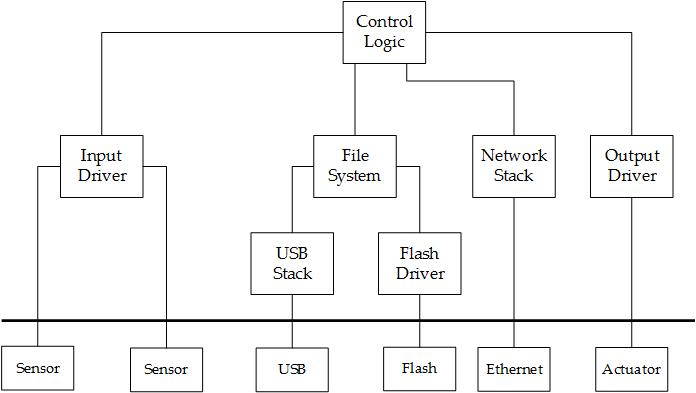
\includegraphics{Figures/Drawing1}
\decoRule
\caption{Test}
\label{fig:sepArch}
\end{figure}
\end{comment}

Spatial separation means that access of physical resources cannot lead to conflicts or corruption. This includes memory access as well as system resources such as hardware peripherals. \cite{Wittenstein.spatial.2017}\cite{perez2013safety}

If shared access to any system resources is necessary, some kind of arbiter needs to be in place to give consistent access to components based on their criticality. 
\subsection{Temporal separation}
Temporal separation is achieved, if it is sufficiently unlikely for any system software to compromise the processing demands of another \cite{Wittenstein.temporal.2017}. 
Managing access to available processing resources is the main part of temporal separation. However, system events and triggers may also require analysis. Excessive interrupt routine run time, for example, can cause processing resources to be unavailable to the main system \cite{Wittenstein.temporal.2017}. 
\subsection{Data integrity and validity}
Data passed through unsafe components has to be either not safety related or protected. Whereas protection refers to ensuring the data's integrity and validity after it has passed through the unsafe components and before it is used in safety related processing \cite{Wittenstein.spatial.2017}.

In practice this requirement doesn't have to be met by the architecture but may be handled in the application software. Nevertheless it is an important aspect that needs to be kept in mind.
\subsection{Certifiable compliance}
It may not come as a surprise that the separation architecture also needs to fulfill these requirements in the eyes of the regulatory bodies, as they are the reason for the architecture's inception.
How this may be achieved differs based on architecture and standard but it needs to be feasible at the very least. 

%----------------------------------------------------------------------------------------

\section{Existing separation architectures}
% TODO Refrain from comparing architectures (or even making qualitative judgments) unless I am building the argument for not analyzing them later. Or I guess only talk about quality of separation (more sources!)
There are some possible contenders for feasible separation architectures. This section will give an overview and narrow down the options for the more detailed analysis in the latter parts of this thesis.
\subsection{General purpose operating system}
Even though this section's title is \acrfull{gpos} realistically it can be substituted with Linux, as other options are usually not considered adequate for embedded devices. But the same arguments should apply to other general purpose operating systems.

With the help of an \acrfull{mmu} or \acrfull{mpu}  a \acrshort{gpos} can achieve the spatial separation of memory between applications. The operating system's access control may be used to limit peripheral access and drivers can arbitrate conflicts. 

% NOTE Am i confusing temporal separation with being able to satisfy real-time requirements?
Temporal separation is usually not possible and may even be counter-productive to the standard processing model of general purpose operating systems, since they are designed to optimize average case performance and sacrifice determinism for it. There are however ongoing efforts to introduce temporal separation as well as the ability to reliably satisfy real-time requirements into the Linux kernel \cite{SiroArthur.2007}.

% REWRITE This section is a bit strange
Undoubtedly these efforts have been at least somewhat successful as Linux has been successfully deployed in some safety-critical systems with hard real-time requirements. One big issue remains however, Linux is massive with several millions lines of code and safety can only be reasoned about on the basis of its "proven in use" status. This is not enough for most regulatory bodies, especially in devices with high criticality, where the benefits of mixed criticality are the most pronounced.

% TODO Fix strange example
Another big problem is damage limitation. While more and more Linux drivers are implemented in user space, a considerable amount still has to be in kernel space . Failures in these drivers can potentially cause a kernel panic, prompting the device to shut down. 

Perhaps Linux, or another, yet unknown GPOS, will be able to solve the mixed criticality problem directly but for now it will be excluded from further analysis, on the grounds that it can not satisfy the separation architecture requirements well enough for a large set of safety-critical devices.
\subsection{Microkernel}
Microkernels are not typically directly deployed on devices but they are very closely related to real time operating systems and hypervisors, architectures that will be introduced later in this chapter. For that reason it is important to review the key difference between microkernel design and traditional monolithic kernel design at this point.
The kernel is the part of the operating system that has complete control over everything in the system. It handles all hardware access for applications running in user space.
\paragraph{Minimality}
\begin{figure}
\centering
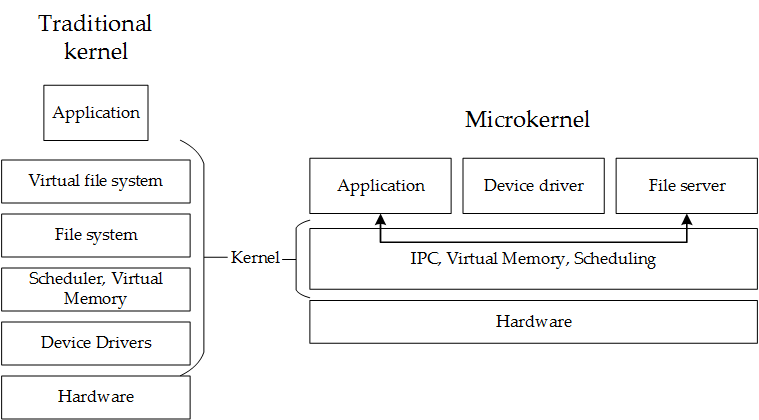
\includegraphics[scale=0.75]{Figures/microkernel_vs_normal.png}
\decoRule
\caption{Traditional monolithic kernel in comparison to a microkernel}
\label{fig:microkernel_vs_normal}
\end{figure}
As the name suggests, the core principle of microkernel design is that of minimality. Meaning, anything that doesn't absolutely need to be in the kernel for the system to function is handled in user space instead. As can be seen in figure \ref{fig:microkernel_vs_normal}, typical monolithic kernels implement everything from the file system to device drivers in the kernel.

A microkernel on the other hand only includes the basic functions like \acrfull{ipc}, virtual memory and the scheduling of processes. This means that shared functionality is implemented in so called \keyword{server processes}. Any process that needs to access the file system for example, can do so over the \acrshort{ipc} mechanism of the microkernel. In figure \ref{fig:microkernel_vs_normal} the arrow between the "Application" process and the "File server" process indicates such a communication.

Microkernels subsequently have much fewer lines of code than monolithic kernels with roughly 10.000 lines of code\cite{Heiser.2016}. Linux as an example of a monolithic kernel has over 15 million lines of code\cite{paul2012linux}. Being comprised of so a little code makes microkernels easier to maintain and refine. This property of microkernels is especially desirable for safety-critical device manufacturers, as it also makes the microkernel verification much easier.

However, with such a reliance on \acrlong{ipc}, much of the system performance is dictated by the speed of the \acrshort{ipc} mechanism. Early microkernels struggled with this but since the advent of the L4 microkernel by Jochen Liedtke \acrshort{ipc} is no longer considered a bottleneck of microkernels\cite{Liedtke.1995}\cite{Liedtke.1996}.
\subsection{Real-time operating system}
% NOTE How do they deal with peripherals?
Providing temporal separation is practically the main purpose of an RTOS, so there are no real problems on that front, and with the aid of an \acrshort{mpu} or \acrshort{mmu} spatial separation is also not a big issue.

One thing to keep in mind though is that a lot of RTOS developers offer no multicore support, which can severely limit the complexity of an application. But perhaps the biggest limitation of application complexity on the RTOS architecture is its narrow target audience.

% TODO Fix example
As a result of this, there is a distinct lack of sophisticated middleware. Especially cutting edge usability technology, like touch gesture recognition, is likely not available on these platforms. At the same time consumers are becoming increasingly adept at recognizing good design and are demanding strong user interfaces \cite{HBR.September2015}.
Additionally, a problem outlined in the section \ref{mixed-criticality} applies to RTOS middleware as well: These libraries have a similarly narrow target audience and can therefore be quite expensive for the functionality they offer.

Although the RTOS architecture remains quite a dominant one, it quickly loses its appeal with growing application complexity. Therefore it will be excluded from further analysis in this thesis.
\subsection{Multicore system}
% TODO Intro: An entirely different approach to separation is separating the components in hardware instead of software
More and more silicon vendors are offering multicore systems with a dedicated safety and a support core. These are usually heterogeneous processors with one application core, like an ARM Cortex A7, and one microcontroller core, like an ARM Cortex M4. Proving temporal separation on these systems is typically not difficult, as the cores are physically separated \cite{Wittenstein.temporal.2017}.

But the cores in these systems share hardware resources like peripherals and memory. Consequently, it can be challenging to show sufficient evidence for spatial separation. An \acrshort{mmu} or \acrshort{mpu} can be useful to enforce spatial separation but it is not a perfect solution, especially for peripherals.
\subsection{Hardware supervised multicore system}
These systems are identical to the ones described in the previous section, except they contain additional hardware to control and arbitrate peripheral access, as well as providing inter-core communication.
Because there is no standard for this, the implementation is entirely up to the silicon vendor. 

Although this hardware supervision has limited functionality, it has a clear advantage over comparable software solutions, like a hypervisor: Hardware is less error prone than software and this is recognized by regulatory bodies. Software typically has to adhere to a more rigorous development and verification process \cite{IEC.2010-3}. It is therefore possible that these systems are cheaper than hypervisors overall. 

This architecture should be considered when designing a safety-critical device but it is still fairly new and a full analysis of it is not in the scope of this thesis.
\subsection{Hardware separated subsystems \label{HSS}}
% NOTE review http://www.ia.pw.edu.pl/~tkruk/edu/eopsya/lecture/eopsy08.pdf and http://www-5.unipv.it/mferretti/cdol/aca/Charts/07-multiprocessors-MF.pdf and if these are viable
% TODO https://witekio.com/blog/introduction-heterogeneous-multicore-processing-architecture/ Read about the need for software support on this architecture
% TODO actually explain what they are
Multiprocessor systems or even completely separate subsystems are the current status quo for dealing with the mixed criticality problem. The multiprocessor architecture should not be confused with the multicore architecture, as it has distinct processors, usually with their own resources, on the same or even different \acrlong{pcb}s (\acrshort{pcb}).

Such a system starts out with perfect temporal and spatial separation because the systems are fully independent. The \mfg{} can then reintroduce dependence in very deliberate and controlled ways, that don't impact the device's safety rating. For example by introducing a dedicated communication channel between the processors. 

% NOTE Is this a qualitative assessment better reserved for the analysis part?
Keep in mind however that, while sharing external peripherals is theoretically possible, it is not commonly done and poses some difficult concurrency challenges. This means that any external peripheral that could theoretically be shared has to be duplicated instead. The same goes for memory.

% TODO Give an example and make an architecture diagram
So what exactly does this architecture look like? Because this is more so a design methodology than a general solution, specific implementations are bound to look very different. In theory there is no limit on the number of processors or how they communicate, that depends on the size of the overall system and the safety requirements. 

More specific advantages and disadvantages of this architecture will be analyzed in more detail later in the thesis.

%----------------------------------------------------------------------------------------
\section{Hypervisor}
Now let’s examine the main subject of this thesis, the hypervisor. Hypervisors originated in networking to optimize server usage and as such there are some misconceptions about their usefulness in embedded programming. These misconceptions will be addressed here but first, we need to take a look at the core functionality of a hypervisor.

\subsection{Hardware virtualization}
The act of hardware virtualization refers to the creation of a virtual machine that
acts like a real machine. A virtual machine is often referred to as a guest and the system it is virtualized on is called the host. The host can either assign hardware to the guests directly or provide them with virtualized hardware components. Virtualized hardware components also behave like their real counterparts from the view of the guest but in reality the host is translating any hardware operations that the guest performs to corresponding operations on the actual hardware. This means the guest can be unaware that it is only a virtual machine and does not have full control over the system.

There are two types of hardware virtualization. Full virtualization and paravirtualization
\subsubsection{Full virtualization}
In full virtualization the virtualized guest is completely unaware that is not a real machine. That means any software that could run on an actual machine can also run on this machine, without any modification.
In theory this can be completely achieved in software but this is very computationally expensive. That is why \acrshort{cpu} designers like Intel and ARM offer hardware virtualization extensions that can accelerate these processes \cite{uhlig2005intel}. However, this also means that if these virtualization extensions are not an option, other ways need to be found to efficiently virtualize a system. Which brings us to Paravirtualization.
\subsubsection{Paravirtualization}
In paravirtualization the software running on the virtual machine is modified, so that it can communicate efficiently with the host platform. To elaborate: A process running atop an operating system can use the available system calls to interact with the hardware below. In a fully virtualized operating system the host system recognizes that an interaction with the hardware has been initiated by the guest, interrupts the communication and takes over. In a paravirtualized operating system on the other hand, the implementation of the system calls has been modified to talk directly to the host system instead of the hardware. This leads to overall more efficient virtualization process because.

In reality there are often hybrid version that take advantage of both paravirtualization and the hardware virtualization extensions of the \acrshort{cpu}. The virtualization extensions are very good at stopping the virtual machines from doing things they are not allowed to and the combination of paravirtualization and hardware extensions increase the efficiency and performance of the virtualization.
\subsection{Hypervisor}
The virtual machine monitor, more commonly referred to as hypervisor, is the software that actually facilitates the communication between the virtualized guest machine and the hardware on the host platform. In a paravirtualized operating system the system calls would need to be adjusted to talk to the specific hypervisor implementation that is used. 

\begin{figure}
\centering
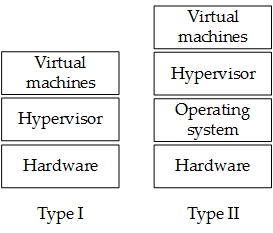
\includegraphics[scale=0.75]{Figures/hypervisor_types.png}
\decoRule
\caption{The two hypervisor types}
\label{fig:hypervisor_types}
\end{figure}
As indicated in figure \ref{fig:hypervisor_types}, there are two types of hypervisors. Type II hypervisors don't interface with the hardware directly and instead delegate any hardware access to the operating system they are running on. This scenario adds additional overhead and necessarily requires an operating system to run on the device. Therefore, Type II hypervisors are not relevant to this thesis.

But even among Type I hypervisors there can be significant differences in what they aim to achieve. Differentiating the two big use cases will be the topic of the following sections.
\subsection{Traditional server hypervisor}
\subsection{Embedded safety hypervisor}







\begin{comment}
\XsecXtion{Embedded safety hypervisor origins}
% TODO Add dat sauce
Now let's examine the main subject of analysis, the embedded safety hypervisor. In this section it will be established where it comes from and some associated concepts. This should get rid of some common misconceptions about hypervisors and their applicability in the embedded sector.
\subsection{Hardware virtualization} \label{hw-virt}
The act of \keyword{hardware virtualization} refers to the creation of a virtual machine  that acts exactly like a real device. Software executed on this machine has no direct access to the underlying hardware resources. Virtual machines are typically called guests, whereas the device virtualizing them is referred to as the host machine
There are two types of \keyword{hardware virtualization}.
\paragraph{Para-virtualization}
Para-virtualized guests run in a separated environment with no direct access to the hardware but their hardware environment is not simulated. That means guest software needs to be modified to run in this environment.
\paragraph{Full virtualization}
In full virtualization the entire guest hardware is simulated, allowing guest software to run completely unmodified.

Doing this kind of simulation entirely in software is very computationally expensive and has only really become feasible with hardware virtualization extensions. These virtualization extensions add an additional level of privilege to the processor, along with additional instructions and hardware enhancements that make virtualization a lot more efficient \cite{ARM.v8.2018}.

Notably, while these extensions were originally limited to high powered hardware, they have since become available in more embedded focused processor lines like the Intel Atom and ARMv7/v8 processors.
\subsection{Original hypervisor use case}
Hypervisors were originally conceived in the 1960s as a way of accommodating multiple users on mainframe computers. After a hiatus they enjoyed their resurgence in the 2000s when the demand on servers rose again. 

So they started out as a way to maximize resource utilization in large servers. However, low resource utilization is usually not an issue in embedded systems, quite the opposite in fact. Therefore these original hypervisors are not the point of discussion for this thesis.
\subsection{Microkernels}
At this point it is useful to make a quick excursion to the realm of microkernels. As the name implies their guiding principal is that of a minimal kernel. Basically, everything that doesn't absolutely have to be handled in kernel space for the device to work is implemented in user space.

This kind of system was exclusive to academia for a long time, until it somewhat matured in the late 90s \cite{Liedtke.1995}\cite{Liedtke.1996}. With this development they had already become attractive to safety-critical device manufacturers and saw some large scale deployment.

\subsection{Unification of the two concepts}
In 2005 an academic debate broke out about the legitimacy of microkernels versus the hypervisors that were around at this time. 
The argument was that, despite their architectural similarities, hypervisors are a special case of microkernels \textquote{microkernels done right} \cite{StevenHand.2005}\cite{Heiser.2006}. Without examining the back and forth that ensued, the result was the addition of hypervisor functionality to existing microkernels \cite{Heiser.2010}. And these hypervisors with a minimal trusted computing base were focused on the safety-critical market, providing safe separation instead of maximum resource utilization.

This does not necessarily mean that microkernel based hypervisors are the definitive embedded safety hypervisor but it is their origin and still by far the most prevalent architecture.

\end{comment}



% Chapter 1

\chapter{The basic safety hypervisor} % Main chapter title

\label{Chapter2} % For referencing the chapter elsewhere, use \ref{Chapter1} 

%----------------------------------------------------------------------------------------

% Define some commands to keep the formatting separated from the content 
%\newcommand{\keyword}[1]{\textbf{#1}}
%\newcommand{\tabhead}[1]{\textbf{#1}}
%\newcommand{\code}[1]{\texttt{#1}}
%\newcommand{\file}[1]{\texttt{\bfseries#1}}
%\newcommand{\option}[1]{\texttt{\itshape#1}}

%----------------------------------------------------------------------------------------

% IMPORTANT Add a section about IPC and interpartition communication
% IMPORTANT Do I talk enough about whether or not developers offer para or full or both?
% IMPORTANT Talk about supported hardware, v7 vs v8 and breadth of platforms

% IMPORTANT Maybe remove the intro fluff?
Now that the differences between traditional hypervisors and embedded safety hypervisors have been laid out, it is time to take a closer look at the embedded safety hypervisor.
For this, a "basic safety hypervisor" will be proposed, that embodies the typical characteristics of a microkernel based safety hypervisor. Where there is no discernible consensus, differences will be highlighted. Both the typical hypervisor architecture and its simplified functionality will be examined.

\section{Architecture}
Since, most safety hypervisors are microkernel based, the architecture for the basic safety hypervisor is also a more in-depth look at microkernel architecture. However, there are differences and additions to the microkernel core that will be explored as well.   

The guiding principle of microkernel design, minimality, has already been introduced in section\ref{microkernel}. But while the academic microkernel representations try to achieve \keyword{absolute minimality}, most real safety hypervisor implementations forego this to add useful features to the kernel. The small trusted code base is still an integral part of safety hypervisors, but with some minor trade-offs. 

% SOURCE Do I need a source for this?
Perhaps, the biggest trade-off is the inclusion of the virtual machine monitor code in the kernel itself. Some hypervisors also relegate this virtual machine control to user-space but it is more typical to see it inside of the microkernel. In reality the virtualization aspect of the hypervisor is almost always a critical component and it therefore makes sense to include it in the kernel verification efforts. 

\subsection{Capability-based access control}
% TODO Explain concept of least privilege
Capabilities are unforgeable tokens that grant access rights to an object. They contain the identification of the object and associated rights, for example read and write.
They can be given to other processes which in turn grants them access according to the capability \cite{Levy.1984}. A capability could be for a specific memory region, a communication endpoint or to a hypervisor \acrshort{api} call.

The capabilities a process has are maintained in a part of memory that it can not write, to stop the process from attempting to forge capabilities. It is however still up to the process to use the appropriate capability for access to reduce kernel involvement.

Capability-based access control has dominated in microkernels because of its flexibility and because it doesn't require extensive kernel involvement. Since, the typical safety hypervisor is an extension of a microkernel, this mechanism has propagated to them as well.

\subsection{Scheduling} \label{hv-scheduling}
All hypervisors implement some form of hierarchical scheduling, where a container task is scheduled that then schedules its children according to a global scheduling algorithm. This is most evident with virtualized operating systems. The hypervisor schedules the virtualized operating system according to the system configuration but how the \acrshort{os} in turn schedules its processes is up to the \acrshort{os}. Hierarchical scheduling can have the benefit of reducing scheduling slack in mixed criticality systems \cite{MalcolmS.Mollison.2010}. 

When it comes to how the container tasks are scheduled there is no single solution that is effective for every scenario. Consequently, the basic safety hypervisor offers different configurable scheduling behaviors. The two most common scheduling algorithms are preemptive priority based scheduling and time-sliced round-robin scheduling. Regardless of which algorithm is used, it needs to be deterministic to enable \acrlong{wcet} analysis. Without deterministic scheduling and \acrshort{wcet} analysis temporal separation can not be guaranteed and the system is unable to verifiably satisfy real-time requirements.

\paragraph{Preemptive priority based scheduling}
% FIGURE This might need one
In preemptive priority based scheduling each process has a priority and processes that are ready to be scheduled are scheduled based on their priority.
The preemptive means that if a process with a higher priority than the currently running process becomes ready to be executed, the currently running process gets interrupted. This ensures that the most critical task always gets the time it needs. If there are multiple processes with the same priority, the first to arrive gets scheduled first.

\paragraph{Time-sliced round-robin scheduling}
In time-sliced round-robin scheduling each process gets a dedicated time slice called a quantum. Figure \ref{fig:round_robin_example}  shows an example with three processes and their associated scheduling windows. If the end of the quantum is reached before the process is done, it gets interrupted and the next process is scheduled.
\begin{figure}
\centering
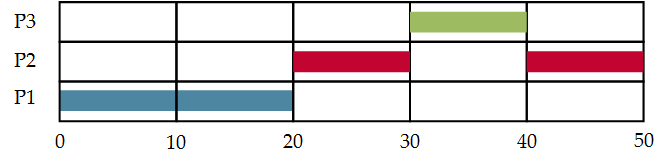
\includegraphics[scale=0.75]{Figures/round_robin_example.png}
\decoRule
\caption{An example for round robin scheduling}
\label{fig:round_robin_example}
\end{figure}

However, these were just the two most prevalent examples and in fact most hypervisors even allow the implementation of custom scheduling algorithms if the provided ones are not sufficient.

Another feature of the basic safety hypervisor is the possibility of multiple scheduling plans. A hypervisor partition with the correct capabilities is allowed to switch the scheduling behavior to one of the plans that was provided at configuration time. For example, if there is an unexpected error the monitoring partition can put the device into a maintenance mode, where only the most critical and recovery processes are scheduled. Another use for this feature is during the boot process where some partitions might need to run uninterrupted for a longer time.

\subsection{Available guest environments}
\subsubsection{\acrshort{rtos}}
Any safety hypervisor can host a \acrlong{rtos} as a guest environment, as it is one of the core objectives to separate real-time, safety-critical domains from the less critical domains. However, as explained in section \ref{hw-virt} (Hardware virtualization) the full virtualization of operating systems is not always available or feasible and in fact many hypervisors don't currently offer full virtualization. That leaves paravirtualization as the only option but paravirtualization requires the modification of the operating system in question. To reduce the barrier of entry the developer of the basic safety hypervisor typically also offers an already paravirtualized \acrshort{rtos} that can be deployed on the hypervisor. 

However, this significantly reduces the possible \acrshort{rtos} options the safety-critical device manufacturer can choose for his application. Since most real-time operating systems are closed source they cannot be modified to work on the hypervisor. This makes the \acrshort{rtos} provided by the hypervisor developer the potentially only viable option and therefore increases the dependence on the developer. What the potential consequences of this are needs to be evaluated based on the context of the situation but it is an important aspect to keep in mind.

\subsubsection{Linux}
An already paravirtualized version of Linux is another standard guest environment. Since, Linux is open-source the pressure of paravirtualization is not an immediate issue. Furthermore, there is less of a difference between versions of Linux than between real-time operating systems by different vendors. It is therefore unlikely that the safety-critical device manufacturer is even interested in using another version than the one provided.

\subsubsection{Native C runtime environment}
For a partition completing a very simple task, running a full-blown operating system is a waste of resources. For that reason the basic safety hypervisor includes a guest environment that is nothing more than a native C application with access to the hypervisor \acrshort{api}. The safety-critical device manufacturer can provide one or multiple C files that then get compiled into a hypervisor process. This process is then scheduled like any of the other partitions.

A possible application of this is a shared device driver. The driver can be implemented in the native C environment and communicate with the other partitions over the hypervisors \acrshort{ipc} mechanism. A more detailed explanation of this will be given in a future section.

%----------------------------------------------------------------------------------------

\section{Functionality}
This section will explore what functionality the safety hypervisor can offer and how it achieves this.
\subsection{Separation}
% IMPORTANT What about the other requirements of a sep-arch?!
The concepts of separation have been introduced in section \ref{separation-arch}. Now it will be detailed how the hypervisor in particular achieves this separation.
\subsubsection{Temporal separation}
How the hypervisor may schedule its partitions has already been explained in section \ref{hv-scheduling}. The most important property of a hypervisor scheduling algorithm that emerged from that was its determinism. If the algorithm is deterministic the device manufacturer can carry out a \acrshort{wcet} analysis, which allows him to reason about the device's temporal separation. The results of the \acrshort{wcet} analysis should show that even in the absolute worst case, the critical partitions still get the time they need to ensure the safety of the device. In all highly critical devices with real-time requirements this is a necessary step to achieve regulatory compliance.

Because the hypervisor has full control over the system it can stop or start processes at will. Through this, the hypervisor can make sure the schedule is kept and no process oversteps its boundaries.

% I kind of need to explain interrupts after I explain device access. And then I can also better explain how they are relevant to temporal separation
Another way for a partition to impact the timing behavior of another partition is through interrupts. Interrupts are the main way external peripherals communicate with the software on the device. They are 



* The ways of scheduling have already been detailed
* The hypervisor can achieve temporal separation because it has full control over the system and can force partitions to stop or start
* The deterministic scheduling behavior is also important to reason about the temporal separation
* Maybe go into more detail
* How are secondary timing problems solved (like interrupts etc.)
    -> I think I may be overcomplicating this issue
\subsubsection{Spatial separation}
% Same as with temporal
On most systems 

* DMA is only possible with IOMMU!

* It achieves this through utilizing the MMU or more rarely the MPU
* Some objects related to partitions need to be saved in kernel memory
* Either, partitions have a kernel memory quota or they can only instantiate objects that were defined at configuration time. This stops them from starving other processes of kernel memory
\subsection{Inter-partition communication}
There are two ways for two partitions to communicate: message passing and shared memory.

\subsubsection{Shared memory}
If two partitions are configured to share memory the hypervisor simply 

\subsubsection{Message passing}

* There are two ways to communicate with another partition: message passing and shared memory.
* In the shared memory case the hypervisor simply maps the same physical memory region into the virtual memory region of both partitions. The partitions then need to take care of everything else themselves. That means the partitions need to make sure they are not overwriting each others data and so on...
* Message passing is done through so called ports. Ports are defined at configuration time and have one source and one or more destinations. There are two types of ports: Queuing ports maintain a FIFO queue of messages that the consumer can take. In sampling ports a new message overwrites the existing one. 
* In the port scenario the hypervisor does have some control over the communication. [Explain what this means and what comes from it]
\subsubsection{User space synchronization}
* Some hypervisors may offer built-in synchronization mechanisms like semaphores to user space partitions
* This is especially useful if two partitions share memory and need to synchronize who is allowed to access it. 
\subsection{Partition privileges}
* At the very least there is two privilege levels. That of a system partition and a normal partition. A system partition is allowed to monitor and change the state of other partitions or the system as a whole. For example, it is allowed to execute the hypercall for shutting down another partition.
* There may also be more granular control where individual hypercalls can be allowed or disallowed
\subsection{Health monitoring}
* First events get detected. There are three types of events:
    -> Events caused by abnormal hardware behavior. The hypervisor is notified of this by processor traps
    -> Events detected and triggered by partition code. These are usually related to assertions or checks.
    -> Events triggered by the hypervisor itself. Usually because of a violation of a sanity check performed by the hypervisor. Either on the hypervisors internal state or that of a partition. This may also include a partition attempting to perform actions it is not allowed to
* A developer can then assign some basic actions that should follow a certain event, like restarting the partition or even the entire system. There doesn't have to be a defined action for everything.
* Simultaneously all events also get reported to the global log stream. Any partition with access to this stream can read it and may take more intricate steps to resolve the problem. This can be performed either as a replacement to the basic action described previously or on top of it.
* Add an image!
\subsection{Device access}
* To control a device, the partition needs control over the corresponding interrupt lines and device registers (typically handled by memory mapped IO on ARM and that or IO ports on x86)
* If only one partition needs access to a device it can be assigned directly.
* If devices are shared an IO Server partition needs to be implemented. It controls the device and gives access to the device over the inter-partition communication mechanism of the hypervisor. 
* Hardware interrupts can be assigned during configuration. 
* The hypervisor also often extends the interrupts there are with his own events. This can be used to notify partitions of hypervisor events like new messages at a queuing port for which they are a destination.
\subsection{Timers}
* Because the hypervisor can obfuscate a partitions view of time compared to if it was running on bare-metal (elaborate what this means), it offers virtual timers.
* The partition may either request the current time or activate a timer and receive an interrupt when the timer expires [...]
\subsection{Static configuration}
% NOTE Maybe this should be at the end of functionality section so I can give better examples for configuration
Configuration includes: 
* hardware resource access
* partition rights (ability to use restricted hypercalls)
* scheduling (with a caveat)
* partitions and what is running on them
* allowed communication paths

Any mechanism to modify a guest's rights at runtime, poses the risk of the system getting compromised, be it accidental or purposeful. For this reason dynamic configuration is not possible in the basic safety hypervisor. The only exception is the switching of scheduling plans by an authorized partition. But in this case all possible scheduling plans need to be defined at system design time and only these predefined scheduling plans can be activated.

That is why these systems are typically statically configured and if configuration runtime is at all possible, it is restricted to reducing privilege. For example, a guest that is allowed to spawn other guests may give them his own rights or less than his own but never more.
* Scheduling plans can usually be switched but only to predefined plans by authorized partitions. This

%----------------------------------------------------------------------------------------
\section{Initial considerations}
% TODO Rename this section
Although the considerations for choosing a hypervisor implementation will be outlined later in the thesis, in section \ref{how-to-decide}, some crucial factors need to be elaborated here to avoid confusion.
\subsection{First- or third-party hypervisor}
A manufacturer has the option to either license a third-party hypervisor or develop his own solution. The development costs of a third-party hypervisor are effectively shared with many parties over the course of many projects, whereas the development costs of a first-party hypervisor are typically only shared over the course of many projects in a single company. However, developing one's own hypervisor provides the maximum amount of control over functionality and development cycle.

Additionally, it means that the best possible subject matter experts on the hypervisor are always available to the manufacturer. But here also lies another big problem: Developing a custom hypervisor not only requires the initial development costs but also the costs of hiring or developing the talent required. A third-party already has these capacities and can therefore also typically go beyond the absolute necessity in terms of functionality.

Ultimately, the more prudent approach is probably licensing a third-party hypervisor but in some cases it may be beneficial to have full control over the environment. 

\subsection{Security}
Security will not be a consideration in this thesis, only a word of warning will be issued. It may seem logical to assume that a hypervisor can provide security as well as safety and while it may not initially be a bad idea to have separation between security-critical and non-security-critical software it is not that simple. A hypervisor offers a much greater attack incentive, as a compromisation of the platform could be used to attack a lot of different devices. It is also questionable whether or not the goals of security and safety align. A manufacturer doesn't want to modify a certified device or at least do it in bulk to minimize the cost of recertification. Building a secure device on the other hand often requires frequent updates to fix newly found attack vectors. So the security of any given hypervisor implementation should not be taken for granted and analyzed with scrutiny.
%----------------------------------------------------------------------------------------

\section{Limitations}
Before getting into the full-fledged analysis it is best to expose some limitations of the current safety hypervisor landscape. 
\subsection{Current hardware restrictions}
Hypervisors are overall still limited to the more powerful \keyword{application processors} and have not really penetrated the \keyword{microcontroller} market. Using a hypervisor is also not possible if a specialized processor, like a \acrfull{dsp}, will be the only processor in the system. Although, this restriction may be lifted in the future.  There are several reasons for the hypervisor's hardware restrictions. 

% PHRASING 
First of all, microcontrollers typically have no \acrshort{mmu} only an \acrshort{mpu} or no memory protection at all. Hypervisors need at least some hardware memory protection, as the corresponding software isolation is far too slow. \acrshort{mpu}s have a limited number of partitions they can isolate and therefore impose uncomfortable restrictions on hypervisor developers and users.

Second, the hardware virtualization extensions are not yet available on microcontrollers. And even though the typical safety hypervisor prefers paravirtualized guests, virtualization extensions are still beneficial for preventing the guest from doing things it is not supposed to. ARM, for example, offers a trap mechanism that allows the hypervisor to disable certain instructions and special registers for the guest \cite{ARM.v8.2018}. 

And finally, a hypervisor is fundamentally about isolating software components from each other. It is more likely that this is necessary on a stronger processor and not on a microcontroller.

However, with all of these restrictions laid out, there are developments that aim to make hypervisors viable on microcontrollers. Read more about this in section \ref{tech-progress}.

\subsection{Effective multicore isolation}
% NOTE Maybe add a graphic
Imagine a system with two partitions, one safety-critical one not safety-critical, that runs on a two-core \acrshort{cpu} with a shared cache between the two cores. During its allocated time the safety-critical partition may fill up the cache with relevant values. Once the non-safety-critical software runs it can evict all of the cache values by populating it with its own values. This can lead to large and potentially unpredictable interference across domains \cite{AlessandroBiondi.2018}.

In the best case this scenario just leads to an excessively pessimistic \acrfull{wcet} analysis and to compensate this the safety-critical partition would get a lot more allocated time than it actually needed, leading to a worse average case performance. There are efforts to solve this issue reliably \cite{PaoloModica.2018}.

%----------------------------------------------------------------------------------------

 
% Chapter 1

\chapter{The key wants of safety-critical device manufacturers} % Main chapter title

\label{Chapter3} % For referencing the chapter elsewhere, use \ref{Chapter1} 

%----------------------------------------------------------------------------------------

% Define some commands to keep the formatting separated from the content 
\newcommand{\keyword}[1]{\textbf{#1}}
\newcommand{\tabhead}[1]{\textbf{#1}}
\newcommand{\code}[1]{\texttt{#1}}
\newcommand{\file}[1]{\texttt{\bfseries#1}}
\newcommand{\option}[1]{\texttt{\itshape#1}}

%----------------------------------------------------------------------------------------

% REVIEW This section has two goals for each want: Explain what the want means and explain why it is important (if it is not self-evident) and maybe explain how it relates to other wants
% NOTE I specifically avoid talking about architecture in this section, maybe I'm actually sabotaging myself with that
The two separation architectures that will be analyzed in \ref{Chapter4} are the hardware separated subsystems architecture (from now on referred to as \acrshort{hss} architecture) and the embedded safety hypervisor architecture. It has been established that both can conceptually solve the mixed criticality problem and now it is time to compare the non-functional criteria of the architectures in question. 

To achieve this a list of criteria will be proposed that will serve as a categorization tool for the analysis.
This list comprises the key wants that manufactures of safety-critical devices want to achieve, when engineering a device. A want can be understood as a business driver for device manufacturers. Fulfilling all wants to the best degree possible, would result in a perfect device. These idealized wants will be used to compare the hypervisor architecture to other device architectures and recommend the features to look for, when choosing a real-world hypervisor implementation.

In an ideal world each want could be satisfied individually but in reality they have complex interactions and need to be carefully balanced. 
Additionally they are not equally desirable for every device. Some devices, for example, might have less potential for causing damage and therefore need to adhere to less strict safety regulations. Therefore choosing the absolute safest architecture is not paramount for the devices success.

\section{Safety}
%[This section is kind of a duplicate of a section in Chapter 1]
It is self-evident that safety is going to be a key want in the engineering process of safety-critical devices. A device that is considered safer is often going to have an edge over that of a competitor. Furthermore, a perfectly safe device protects the manufacturer from expensive lawsuits.

Because of this, it is often beneficial for the manufacturer to ensure higher safety than required. However, in terms of economic viability, there are even more critical wants, as will become clear in the next section.

\subsection{Regulatory compliance}
%[This section is kind of a duplicate of a section in Chapter 1]
To protect the end-customer of safety-critical devices, most regulatory bodies implement rules that govern how safety-critical devices have to be engineered and what quality level they have to fulfill.
Failing to achieve this is even more costly than lawsuits, since it will disallow the manufacturer from selling the device in the first place. The regulatory bodies then allow the manufacturer to make adjustments to his compliance documentation and resubmit the device. For most regulations it’s not just enough to prove that the end result has a high level of quality, the engineering process itself needs to be of high quality as well. This means that it is normally completely infeasible to make a device safe in the eyes of the law, if it has not been developed with this goal from the start. 

And while regulatory bodies almost always find some problems in the compliance, fixing them will cost additional money and time and getting it right the first time is therefore desirable.

\subsection{Real-time requirements}
% NOTE I am only looking at it from a safety perspective but there can also be usability implications.
As a special safety requirement, some devices have to guarantee that an event can be completed in a certain amount of time \cite{shin1994real}. This has a significant impact on the entire device architecture, from the hardware, through the operating system to the actual application. Which is why it deserves special consideration.

The actual time frame that has to be guaranteed can vary wildly and whether it is 500ms or 50ns does have an impact on how the device needs to be implemented. However, the analysis in the latter parts of the thesis will focus more on the core architectural differences that make satisfying this requirement possible in the first place. 

\section{Lowest possible cost}
% TODO Remember to include the distinction between initial and life-cycle costs
% NOTE Is this assumption necessary for any point I will make?
% NOTE Maybe make it clear that the actual Kano analysis is not necessary. I'm just making a point on the theoretical level
There are conceivable edge cases where a company might decide to go through with an unprofitable device for strategic reasons. Prestige customers or the possibility for profitable long-term business come to  mind. But in the interest of simplicity this thesis will assume that the manufacturer wants every project to be directly profitable.

With this assumption in mind, every other want needs to be realized with the pressure of cost in mind. To analyze the architecture effects, cost will be split into multiple subcategories:
\paragraph{Development costs}
The biggest part of the development cost is based on how many developers work on the project, how  much they are paid and for how long they are working on the project. This is true for both hardware and software but the specific numbers may differ. If third-party software is used, the corresponding license costs are another factor. 
\paragraph{Hardware costs}
How much the hardware in the device costs can be very important in some projects. Most costs associated with development are one-time costs, while hardware costs have to be paid for each produced unit. Therefore, this is an especially important factor in devices that are produced in high volume.

\subsection{Optimal time to market \label{optimal-ttm}}
Time ultimately costs money but a faster development process can have additional benefits that will be examined in more detail. To help with this, we will lean on the categorization of functional requirements established by the Kano model \cite{KanoNoriaki.1984}\cite{ElmarSauerwein.1996}. According to the Kano model there are three types of functional requirements.
% TODO Add graph
\paragraph{Must-be requirements} \textquote{If these requirements are not fulfilled, the customer will be extremely dissatisfied. [...] Fulfilling
the must-be requirements will only lead to a state of "not dissatisfied"} \autocite{ElmarSauerwein.1996}

\paragraph{One-dimensional requirements} \textquote{With regard to these requirements, customer satisfaction is
proportional to the level of fulfillment.}\autocite{ElmarSauerwein.1996}

\paragraph{Attractive requirements} \textquote{Attractive requirements are
neither explicitly expressed nor expected by the customer. Fulfilling these requirements leads to more than proportional satisfaction. If they are not met, however, there is no feeling of dissatisfaction.}\autocite{ElmarSauerwein.1996}

This analysis is only based on the theoretical concepts and does not mean a Kano model analysis needs to be carried out. Furthermore, one-dimensional requirements will not be further considered as they can be simplified to be must-be requirements below zero satisfaction and attractive above zero satisfaction. 

% TODO Maybe elaborate on TTM benefits
Projects typically have an ideal time to market \cite{clark1989project}\cite{stalk1988time} that maximizes potential revenue and units sold. If some functionally takes less time to implement, more can be achieved within this ideal timeline. Especially, attractive requirements can be more easily considered and give the manufacturer an edge over his competitors. If the optimal time is missed and less overall units are sold the manufacturer can not take proper advantage of the economies of scale. More overall produced units means more components can be bought, which drives down the price. One way to reduce the time it takes to include functionality is to use third-party software, either free open-source or paid for. 

\section{As few faults as feasible}
% TODO Also talk about fault severity. If an architecture doesn't reduce the total amount of faults but reduces the amount of faults that lead to defects or severe defects, it is still a win
% NOTE what is "possible"
% NOTE I exclusively mention software faults here!
% NOTE I think I accidentally took away some content from "Maintainability"
Faults are undesirable in any engineering environment but they are especially undesirable in safety-critical devices. They are inherently unpredictable and can incur significant costs, both directly through the cost it takes to find and fix them and indirectly through customer dissatisfaction and damage caused.

Reducing the amount of faults to a minimum has multiple dimensions:
\paragraph{Reducing the frequency of fault implementation}
% TODO Go into modular architecture benefits once that section exists 
It is still the common understanding that all non-trivial software that isn't formally verified will contain faults \cite{Klein.2009}. But in the decades since the software crisis it has become evident that development processes and architectures can have a positive impact on how many bugs are built into the software \cite{Randell.1996}.  Measures that reduce the likelihood of fault implementation can avoid all costs associated with the faults entirely and can therefore bring the biggest improvements. 
\paragraph{Finding faults effectively}
% TODO Go into modular architecture benefits once that section exists 
But not just frequency of fault implementation can be improved by a strong architecture. After a significant period of sophisticated testing, almost all "hard" bugs will be found. That is bugs that can be found easily and reliably with standard techniques. Most of the remaining bugs will be "soft" bugs, often called "Heisenbugs" \cite{Gray.1986}. Named after the Heisenberg uncertainty principal because they often disappear when you look for them. Typically this is because the bugs are caused by complex interactions and race conditions that don't necessarily appear in the software debug environment.

A system that can aid the discovery of these bugs, maybe through clever compartmentalization or logging, can save time and money for the manufacturer.
\paragraph{Fixing faults effectively}
% NOTE Should this part be in the analysis instead? Maybe I should just say why its important. -> At the very least make sure that this point gets picked up in the analysis.
% REWRITE Once the software architecture bridge has been moved to chapter 3
% NOTE There is also more to this than just modularization making changes easier
Once a fault has been found it also has to be corrected. Software that is easy to modify usually utilizes the virtues of information hiding and modularization. Changing any line of code only has the readily apparent effect and no other part of the software is invisibly dependent on it. If this property is not present in the device, there is a greater risk that new faults get introduced while trying to resolve the original fault. 

How many work hours ultimately need to be invested into fixing the fault, depends on the fault but a perfectly modifiable device will reduce the associated risks.
\subsection{The lowest possible fault severity}
% TODO Agree on a definition for fault, error, defect etc. and then come back to this
% UFF Laboured...
Having the smallest amount of faults possible is great but ideally these faults also cause the least amount of damage possible. Actually, a part of fault severity is already included in the definition of criticality, as criticality is the function of possible damage and likelihood. Apart from the damage a fault may cause, its severity can be further broken down into the two categories below. In fact, improving fault isolation and fault tolerance can reduce the criticality of a safety function by reducing the maximum possible damage a fault may cause.

\paragraph{Fault isolation}
% PHRASING first sentence 
Ideally,  a fault only affects the parts it absolutely has to. An unrecoverable defect in the USB driver, for example, would ideally only cause the USB port to stop working and nothing else. A negative example of this would be if the fault instead caused a kernel panic that prompted the entire system to go down immediately.
\paragraph{Fault tolerance}
% TODO Maybe at least explore some examples
Even in the event of a fault, a lot of safety-critical systems have to continue functioning. This often involves recognizing the fault and reacting to it or even complete redundancy of the system.

\section{Human factors}
Even human factors can not be left unconsidered in such an important architectural decision. First and foremost there is the importance of the manufacturers employees. If they are unhappy with their work, they are more prone to errors.

One example of this could be a difficult to work with piece of software that requires performing many repetitive tasks. Repetitive tasks are shown to decrease efficiency and increase the chance for mistakes \cite{Wyatt.1937}. Additionally, depending on the cause for the dissatisfaction it can also be indicative of problems that could them self introduce errors. In this instance the employee dissatisfaction is only an indicator for a hidden root cause.

% TODO Incorporate both of these points into the analysis, if they are not there already
Another aspect of this are the end customers of the safety-critical device manufacturer. Their desire for a high quality device is already encapsulated in the other key wants, this want is about more indirect customer demands. Two relevant representations of this are device design and ecological footprint. Customers are becoming increasingly aware of good design \cite{HBR.September2015} and this affects both the \acrfull{gui} design as well as the physical design. 

Ecological footprint is also becoming increasingly important for a companies public image. A development process that can reduce waste and used resources can help realize this want.

% first version
\begin{comment}
This \textit{want} may seem odd at first [Is saying this unprofessional?] but employees are the ones that are ultimately responsible for the success and failure of the project.

If we take software tools as an example: The software could be difficult to work with or include many repetitive tasks. Repetitive tasks are shown to decrease efficiency and increase the chance for mistakes \cite{Wyatt.1937}. Additionally, depending on the cause for the dissatisfaction it can also be indicative of problems that could them self introduce errors. For example a software tool that is overly complicated. In this instance the employee dissatisfaction is only an indicator for a hidden root cause.

An employee that is unsatisfied with his job, for whatever reason, is also more likely to leave the company. If the person was critical to the project this can have hugely detrimental effects. Furthermore, if enough key people leave, the entire project can be endangered. 
\end{comment}

% ---- OLD RISK ----
\begin{comment}
% Beginning of rewrite
Understandably, the world of safety-critical device manufacturers is a conservative one indeed. [...]

% REWRITE This section
Imagine two device architectures \textit{A} and \textit{B}. Architecture \textit{A} has the potential to create perfectly reusable software, much better than architecture \textit{B}. But it is possible that \textit{A} introduces expensive safety problems later in the development process.
In this case architecture \textit{A} has a much higher associated risk but also  some positive variance. This example is very abstract and some more concrete architectural risks will be introduced in future sections. 

Which risks are considered "worthwhile" is very dependent on other circumstances and even in this example it is not clear what would be the better architecture (even assuming that they have no other defining criteria). However, just considering the possible risks of architectures can give important insights into when they should be used.
[Example is confusing and section seems incomplete]
\section{Future-proof design}
Whenever there is an associated hardware , future-proof design is especially important. Software can be reproduced and shipped with practically no cost but devices can not. Any features that have been forgotten can only be added once the next major hardware revision is released.

Safety-critical devices are particularly notable in this respect, since they are often very complex and have an expensive engineering process. Airplanes are typically used for 3 decades and hospitals have notoriously tight budgets and have to squeeze as much lifetime out of their devices as possible. 
\end{comment}
\subsection{Extendibility and maintainability}
Nowadays it is becoming increasingly more plausible that it is possible to deliver software updates to an embedded device \cite{OndrejKachman.2016}. Along with the previously mentioned long life cycle it is a beneficial strategy, if not an expected service, to provide updates for the device.
If the device's hardware supports it, new features could be implemented but the currently more typical scenario are updates of a more basic kind. Meaning, bug fixes and security updates.

In any case an easily extendable device can have significant benefits.
\subsection{Reusability}
This \textit{want} relates to another aspect of future oriented design. Towards the end of a device's life cycle, manufacturers are starting to plan the next generation with upgraded hardware and new features. If the software from the previous generation is reusable and suitably portable, a lot of time and money can be saved on this new generation.

Another scenario for this is the \textit{device platform}, where there is a core device and several variations for different markets. In this example it is presumably even easier to profit from reusable software.

The next device generation and another device on the same platform have the advantage that they presumably share most of the business logic with the original device. That makes reusing a lot of the software plausible. However, if the software is reusable, suitably generic software could conceivably even be used in entirely different devices.
%----------------------------------------------------------------------------------------

\section{Conclusion}
In this chapter it has been proposed what criteria are most important for safety-critical device manufacturers and why. Using these wants as categories it will now be analyzed how the hypervisor architecture stacks up against the well established \acrshort{hss} architecture.
% Chapter 1

\chapter{Analysis of how the architectures satisfy the key wants} % Main chapter title

\label{Chapter4} % For referencing the chapter elsewhere, use \ref{Chapter1} 

%----------------------------------------------------------------------------------------

% Define some commands to keep the formatting separated from the content 
\newcommand{\keyword}[1]{\textbf{#1}}
\newcommand{\tabhead}[1]{\textbf{#1}}
\newcommand{\code}[1]{\texttt{#1}}
\newcommand{\file}[1]{\texttt{\bfseries#1}}
\newcommand{\option}[1]{\texttt{\itshape#1}}

%----------------------------------------------------------------------------------------
% REWRITE Feels a bit lacking and doesn't really get to the point (Probably because I haven't entirely found the point yet)

The two  architectures that will be analyzed are \keyword{hardware separated subsystems} and the \keyword{embedded safety hypervisor}. It has been established that both can conceptually solve the mixed criticality problem and now it is time to compare the non-functional criteria of the architectures in question. 

First of, the most crucial differences between the two architecture will be elaborated. Then it will be explored how these differences can help or hinder the satisfaction of the \keyword{key wants} of safety-critical device manufacturers established in chapter \ref{Chapter3}. 

\section{Crucial differences}
\subsection{Hardware or software}
Even though the hypervisor can be supported by hardware the separation is still fundamentally implemented in software. In the\acrshort{hss} architecture on the other hand, separation is entirely realized through hardware, or rather lack of shared hardware. This does not mean that a device with the \acrshort{hss} architecture does not contain software, only that the software is limited to the business components of the device.

% TODO Try to find sources for these claims and explain them more deeply
% NOTE Have I ever explained the difference between random and systematic faults
% IMPORTANT This is missing something
There are a number of differences between hardware and software developments that are relevant to this analysis. 
\begin{itemize}
\item Software is easier to change than hardware. 
\item Hardware complexity is restricted by physical laws. Software complexity is only really limited by our ability to manage it.
\end{itemize}
\subsection{Specialized or general}
A hypervisor is a general software solution that is meant to be usable in a lot of cases with minor modification. It is often procured from an external company and not developed in-house specifically for a project.

The \acrshort{hss} architecture is technically a very general methodology but each implementation is a specialized solution for one project or project line. This does not mean there is no overlap between different projects using hardware separated subsystems but that there is little room for reuse of the architecture implementation.

% TODO Is there more to add?
An advantage of a more general solution is that the one-time development costs can be spread across multiple projects, or in the case of third-party solutions, across multiple customers.   

\subsection{Distributed or centralized system} \label{distributed-or-centralized}
The \acrshort{hss} architecture ultimately achieves its separation through being a distributed system. In contrast, a hypervisor is a centralized system with added separation between the partitions. In the special case of hardware separated subsystems the subsystems are typically also heterogeneous, which leads to a number of potential disadvantages.
% NOTE Verify these claims
\begin{enumerate}
\item Partition binaries need to be compiled differently.
\item Partitions have distinct bootstrapping processes.
\item Debugging the system as a whole is not possible.
\item The asynchronous nature of partitions, along with point three, can lead to errors that are very difficult to replicate.
\end{enumerate}
This does not mean debugging problems in hypervisor implementations are impossible, just that they can be feasibly addressed in a centralized system. The hypervisor as an entity can have a complete view of the system and therefore the developer can provide appropriate tooling to debug hypervisor partitions or even the hypervisor itself.

\subsection{Advanced fault-tolerance} \label{advanced-fault-tolerance}
% NOTE Name?
% TODO Mention that DSP can not be used with a HV at the moment
Advanced fault-tolerance is referring to the three practices of replication.
\paragraph{Replication} Providing an identical replica of a system component or the entire system that computes the output in parallel. The replicated systems may only act as a supervisor to the primary system or have an influence on the final output via a quorum.
\paragraph{Diversity} Virtually the same as replication except that the additional systems are not identical to the primary system. They can differ in both hard- and software or just one of the two. This approach requires more effort but can reduce the probability that both systems have the same fault. 
\paragraph{Redundancy} In this approach the identical replica, instead acts as a backup in case of a failure in the primary component.

While this does share the key characteristics with the hardware separated subsystems architecture the intention is a different one. 
Replication has the sole purpose of increasing the fault-tolerance and subsequently the safety of the system, while the \acrshort{hss} architecture is focused on separating components of differing criticality to reduce effort and cost among other things.

The hypervisor on the other hand can only provide software diversity on its own and can impede efficient and effective replication. Typically only the most safety-critical parts of the device would be made redundant but on the hypervisor architecture they are all consolidated onto one hardware platform. This means that either the entire hypervisor with all partitions is replicated, forcing the manufacturer to also copy the non-critical partition. Or only parts of the software are replicated and run in an additional partition. While this is a lot cheaper it is also not nearly as effective as hardware replication.
\subsection{Cost of adding a partition}
The core of the \acrshort{hss} architecture is that every partition is its own computation domain with separate resources. In the hypervisor architecture the most expensive partition to add is the second one, as it involves accommodating for the hypervisor in the first place. Any partition that is added beyond the second just requires the appropriate amount of memory and computational resources to be available. Naturally, there are limits to this as each partition also introduces some overhead in terms of kernel memory and process switching times.  Furthermore, a partition requires a certain amount of resources to even do useful work in the first place.

% TODO Consider the fact that if the hypervisor only supports operating systems there is also overhead associated with that

% NOTE This sounds like it is overall more expensive
So only looking at the final unit cost, adding a partition to a hypervisor is cheaper than adding a partition to a hardware separated subsystem. The more far reaching effects of this will be analyzed later.

\section{Safety and regulatory compliance \label{safety-analysis}}
 Let's move on to the first and most important want, safety and regulatory compliance. 
 \paragraph{Hardware redundancy}
 % TODO Fix terminology and think if this is even a separation architecture
 % TODO Make this a crucial difference and change refs to "safety-analysis" to point to that section
 % TODO Include point about the HV being a single point of failure
 % NOTE I am mixing redundancy with fault detection
 At the highest criticality levels redundancy is often required to reduce the devices criticality level. Alternatively, a second partition may supervise the first to detect erroneous output, even if it can't fully replace the first in case of a failure. With Moore's law coming to an end transistors have achieved staggeringly small sizes. One unintended consequence of this is that complex processors have become more prone to random errors \cite{Constantinescu.2003}. Consequently, this scenario is becoming more relevant.
 
 % TODO Make an architecture diagram highlighting my point
 A hypervisor can at most offer software redundancy with two partitions running distinct software that achieve the same functionality. These partitions can then act as a fallback, supervise the other partition or operate in tandem and vote on each output. Hardware separated subsystems are much more confident in achieving this safety as they can offer both hardware and software redundancy. 
 
However, this use case is different from the pure mixed criticality problem. If there is any type of redundancy, both partitions are still at least somewhat responsible for the safety functions of the device. But with mixed criticality we often talk about being able to integrate basically unverified convenience functionality, like a complex GUI running under Linux, into the device. That would not be plausible in this use case unless another partition is added and as has been stated earlier, adding another partition is more expensive in the \acrshort{hss} architecture.

% NOTE This makes more sense here but kind of violates the want structure  because there is already a cost want
\paragraph{Certification cost}
% TODO Figure out the hardware software difference and finish this section.
% IMPORTANT include a part about hardware vs. software! And differentiate between certifying hypervisor and business software

% Is this a mute point?
Since the lowest level of the hypervisor needs to be reimplemented for every platform, the hypervisor also needs to be reverified for every platform. However, this does not need mean the previous efforts are irrelevant. A case on regression analysis can be built.
Furthermore, a project specific risk analysis also needs to be carried out regardless of the hypervisors certification status.

Each \acrshort{hss} implementation needs to be verified from scratch but as stated in section \ref{HSS} providing sufficient evidence for separation should be much easier. The entire point of the architectures separation is that there is almost no avenue for influence to occur. Only through specifically implemented and controlled communication paths.
% NOTE Think about that last point

Ultimately the amount of control a system designer can exert on a device with the \acrshort{hss} architecture, the fact that is hardware and not software and it separation mechanism should make a \acrshort{hss} architecture cheaper to get approval for in most cases.

% TODO Add recertification costs here?

\paragraph{Impact of scalability on safety}
The scalability problems of the \acrshort{hss} architecture have already been discussed but not their implications on safety. \acrlong{emc} or \acrshort{emc} for short is quite important for safety-critical devices, especially for ones operating in explosive atmospheres. Additional processors require more power and more cables that can act as antennas. This introduces more \acrshort{emc} challenges that need to be tackled by electromagnetic shielding and other methods. If they are not properly addresses they can cause high redesign costs at the end of the development cycle.

Additional hardware components also introduce more points for random failure and degradation, which may further reduce a \acrshort{hss} device's safety with a growing amount of partitions.
% NOTE Maybe mention HVs multicore support

\paragraph{Additional safety features}
A hypervisor is a general software solution that can afford to have additional safety features along with its separation. By design it has a full view of the system and its events, a lot of implementations offer features like \keyword{Health monitoring} or \keyword{logging}. This can enable the device to detect and react to faults as they occur and positively impact its safety rating.

\paragraph{Conclusion}
The \acrshort{hss} architecture provides the best possible safety and separation, even though this performance may degrade, if more subsystems are added. But ultimately a hypervisor only needs to be safe enough, not safer than \acrshort{hss}. It is possible that hypervisor technology is not yet mature enough to compete in the most critical environments where absolute certainty is required. Therefore, if the hypervisor architecture is being considered for a future project it should be clarified, whether or not it can pass the certification. If it turns out to be sufficient however, the manufacturer can take advantage of its other benefits detailed in the following sections.


%----------------------------------------------------------------------------------------

\section{Lowest possible cost}
\paragraph{Development costs}
Unfortunately, there is no general quantitative analysis of the development costs associated with the two architectures. Hypervisor developers do not make their license costs, or even their license models, public, as they are subject to negotiation and dependent on other factors like amount of produced units among other things. Since the \acrshort{hss} architecture is usually a custom solution its price is equally difficult to predict. Nevertheless, there are some arguments that can be made on the relative price differences. 

Hypervisors, whether written in-house or by a third-party, are meant to be general solutions, applicable in many projects. In contrast, the \acrshort{hss} architecture is reimplemented for each device or device family. This gives the developers more control but general solutions have a significant benefit: The cost of the hypervisor will be spread across multiple projects, or in the case of a third-party hypervisor even across multiple customers. Another benefit of using a third-party hypervisor is that in a long-term relationship with the developer, prices may be favourable for the manufacturer.

But there is a problem with general solutions: It is possible that the manufacturer is forced to pay for functionality he would not have included in the device, had he used a specialized architecture. 

In the hypervisor architecture the manufacturer also needs to pay the potential license costs for the operating systems, running on the device, on top of the original hypervisor license costs.

\paragraph{Hardware costs}
% TODO Read this again.
Each additional subsystem in the \acrshort{hss} architecture will add another processor, memory and peripherals and consequently increase the device's hardware cost significantly. A hypervisor would usually require a more advanced processor with slightly more memory and computational power but this is less expensive in most cases [source Roy Master thesis?]. Additionally, most peripherals can be shared between hypervisor partitions with some exceptions.

\subsection{Optimal time to market}
In section \ref{optimal-ttm} the concepts of \keyword{attractive and must-be functional requirements}, as well as the\keyword{ideal time to market} have been introduced. Now it will be analyzed how each architecture can impact the time to market and therefore not only the unit cost of the device but also what features are feasible to integrate.

Both architectures have in common, that they can enable the use of unverified third-party or even open-source software for the less critical  components of the device. However, the hypervisor has the advantage that partitions are cheaper to add. This means it is more likely that the cost of adding a partition is outweighed by the benefits of satisfying more attractive functional requirements. Assuming that the license cost of the hypervisor does not negate this benefit for a specific project.

Another way for the architectures to impact the development time is the implementation time of the architecture itself. Not only is the \acrshort{hss} architecture typically implemented individually for each project, but some development efforts even have to be duplicated. If the subsystems are heterogeneous the \acrfull{hal} will also need to be implemented multiple times. 

Assuming that the hypervisor is developed by a third-party the development efforts of the device manufacturer are reduced. They still need to potentially modify the hypervisor to run on the target platform and configure it but the separation itself is taken care of.

% TODO Find a better way to phrase this
One last type of time saving factor is the impact on the development process itself. These are, however highly dependent on the actual situation and the differences listed here are to be understood as criteria too look out for and not guaranteed benefits of a hypervisor: Oftentimes the software team can't begin work until the hardware team has assembled a first prototype of the device. The hypervisor architecture has both a less complex hardware and significant hardware abstraction. Consequently, software development could begin sooner both in a simulated environment and on the first prototype. Additionally, a hypervisor developer is able to provide a fully fledged \acrshort{ide} to make configuration of the architecture easier.

%----------------------------------------------------------------------------------------

\section{As few faults as feasible in the end product}
There are two ways for an architecture to influence the faults in a device. First, the architecture itself may be faulty. Second, the architecture may impact the faults in the business software on top of the architecture positively or negatively.

% https://docs.microsoft.com/en-us/previous-versions/msp-n-p/ee658124(v=pandp.10)
There is a key principle of how a separation architecture might influence faults in the business software running on top: The basic attributes of a separation architecture are similar to the principles of good software architecture design below. Those have been successfully used to reduce faults and manage complexity in software projects over the past decades [source]. Even the smallest possible separation architecture, is ultimately about information hiding and enforcing the separation of concerns.
% TODO Explain the ones I rely on and cut the ones that don't apply
\begin{enumerate}
\item Separation of concerns
\item Single responsibility principle
\item Principle of least knowledge
\end{enumerate}
The hypervisor architecture can have an advantage in fulfilling these principles because of the lower cost of adding a partition. Especially, if partitions do not have to operate an OS and can rely on the native hypervisor \acrshort{api} instead, more granular separation becomes feasible. However, this ultimately depends on the configuration of the hypervisor and is not a necessary benefit.
What concrete benefits can come from this will be discussed in the following sections.
\paragraph{Faults in the architectures themselves}
General solutions, like the hypervisor, are reused over a long period of time and consequently there are more chances to fix faults in the original implementation. For example, faults found by static analyzers in the Linux driver code have decreased significantly over the past 10 years \cite{palix2011faults}. Granted, hypervisors do not enjoy the same popularity as Linux but they also contain much less code and safety hypervisors are used by very scrutinous  parties that are perhaps more likely to find faults.

% NOTE This feels a bit out of place. Maybe a crucial difference or go to safety section (or there is some overlap and I need to decide)
But hypervisors have a significant disadvantage, they represent a single point of failure in the system. This probably has the biggest implications for security but is also very important for safety. For some systems a single point of failure might not be tolerable at all for others the hypervisor's unerring functionality just needs to be sufficiently evidenced. Perhaps even going as far as \keyword{formal verification} [source seL4].

% TODO Include hardware vs software points

% NOTE Is "reducing" the best term?
\paragraph{Reducing the frequency of fault implementation}
Complexity breeds faults \cite{nguyen2017impact}, so one way to reduce the amount of faults implemented is to reduce the complexity of the device. If configuration of the separation architecture is carried out in a sensible manner each added partition will reduce the complexity of each individual partition. Both architectures enforce the modularity of the components and typically provide vetted methods of communication but partitions can be added more cheaply in the hypervisor architecture.

If a third-party hypervisor is used the safety-critical device manufacturer will not have the same amount of familiarity as with a solution that is designed in-house. This could lead to more configuration errors that ultimately leave the device vulnerable. But the hypervisor developer can mitigate this problem by providing strong documentation and development tools.
% NOTE Is there any impact by the centralized vs. decentralized difference?

\paragraph{Finding  faults effectively}
% NOTE I really can't keep reiterating that partitions are cheaper in the HV
Because faults are isolated to the partition they occur in more partitions means that the amount of code that could be responsible for the fault is reduced. Consequently, finding the fault will be sped up.

One big potential problem with third-party hypervisors though is that the source code might not be available. This can complicate the debugging process, if there are faults in the hypervisors or there are conditions that trigger faults in the business software. 

When it comes to the decentralized nature of the \acrshort{hss} architecture, its effects on effective fault discovery have already been described in section \ref{distributed-or-centralized}. Similarly, the hypervisor developer has an opportunity to provide tooling that aids the debugging process, trough tracing internal hypervisor and partition events.

\paragraph{Fixing faults effectively} \label{effective-fault-fixing}
While the architectures might not directly influence how easy it is to fix faults, apart from the benefits of a modular architecture outlined earlier, they can ease the cost of recertification. Once an update for the device has been created, regression testing needs to be performed to make sure the fix did not corrupt any other software components. Typically not all tests are rerun, instead the manufacturer can provide evidence for why certain tests can be excluded. A separation architecture can provide free evidence for this analysis and reduce the costs associated with releasing device updates.

On another note, if a third-party hypervisor is used, faults in the architecture would most likely have to be fixed by the original developer, increasing the dependence.

% * Hypervisors might allow for a more easily testable product [Why though? Can I back this up?]
\subsection{The lowest possible fault severity}
\paragraph{Fault isolation}
Fault isolation is one of the key pillars of separation architectures, as it reduces the chance for catastrophic failure and enables graceful degradation. More partitions means that a more graceful degradation is possible, potentially smoothing the user experience. If in a system with a critical and a less critical partition, the less critical partition catastrophically fails, all associated functionality will no longer be available as well. The subjects of the device might not be in immediate danger but usability would be greatly reduced.

At this point it is important to reiterate that the hypervisor represents a single point of failure and compromisation could lead to a compromisation of the entire system. The \acrshort{hss} architecture can not only offer features like redundancy but also offers much more control with any single points of failure being avoidable. Therefore, extremely high risk devices are most likely better off with its separation.

\paragraph{Fault tolerance}
The hypervisors centralized view of the system present the opportunity for detecting faults and other events of interest in each partition. It can recognize when a partition has shut down unexpectedly and either take action itself or delegate a manufacturer created partition to deal with the problem.

But as stated in section \ref{no-redundancy} the hypervisor can potentially fail to safeguard or even recognize hardware errors. Furthermore, it can only provide software diversity on its own.

%----------------------------------------------------------------------------------------

\section{Human factors}
Ease of use for a hypervisor is mostly dependent on the development tools provided, and therefore hard to generalize. The most sophisticated examples might have a fully fledged \acrshort{ide} that aids the configuration of the hypervisor and perhaps even fully integrated debugging and tracing for devices currently running a hypervisor. % TODO add a counter example

However, hypervisors are still a new technology and especially in such a conservative industry as safety-critical device manufacturing there is bound to be skepticism. This could increase the technological risk on a project using the architecture significantly and irritate engineers on the project.

The effects of the decentralized nature of the \acrshort{hss} architecture, laid out in section \ref{distributed-or-centralized} not only complicate debugging but can also decrease employee satisfaction and increase the chance for human errors.

Finally a slightly different point: Environmental protection is becoming increasingly more important for consumers and companies as a method of differentiation from competitors. The \acrshort{hss} architecture not only increases the size of the device, relative to the hypervisor architecture but also the material used. This increases the ecological footprint of the device and can compromise an otherwise sleek design.

%--------------------------------------------------------------------------------------

%----------------------------------------------------------------------------------------

\section{Reusability}
The hardware abstraction provided by the hypervisor can increase the amount of software that can be reused for the next generation or even other projects. Not only can the business applications be programmed for one of the guest environments but the \acrshort{api} can provide further abstraction from the hardware and the communication with other partitions.

Since the \acrshort{hss} architecture itself is typically implemented by the device manufacturer reusing it is also of interest. This can pose considerable problems however, because the entire hardware platform is typically created specifically for one project only limited reuse is likely.

%----------------------------------------------------------------------------------------

\section{Extendibility and Maintainability}
% NOTE I have written this a million times by now
Not only is software more easy to modify than hardware but adding partitions is also cheaper in the hypervisor than in the \acrshort{hss} architecture. Therefore, it is conceivable that another partition may be added in a future software update, assuming that the necessary computational resources are still available on the platform. 

A point that applies to both extending the device as well as resolving bugs is one introduced in section \ref{effective-fault-fixing}. Any separation architecture can make regression testing significantly cheaper and consequently also the deployment of any update. 

%----------------------------------------------------------------------------------------

\section{Conclusion}
Probably the most important takeaway from this analysis is that it is inconclusive. There are two reasons why this is the case: Firstly, because there are unknown variables, like the typical cost of a hypervisor license. Without any basis in cost no general assessment can made of the worthiness of the hypervisor benefits. Therefore this analysis needs to be completed either by further research, or more likely, by a safety-critical device engineer using this thesis as a guideline. This also ties into the second reason: the key wants are a useful tool for categorization of the benefits, but with safety-critical devices being as diverse as they are, no general claims can be made on their relative importance for a real-world project. Ultimately, this means the benefits and drawbacks that crystallized in this analysis need to be viewed as likely outcomes and possibilities that require a concrete analysis, should the thesis be used as a decision making aid. The future section \ref{ref-projects} will attempt to lift at least some of the uncertainty.

% KEEP IT SHORT AND SIMPLE! DO NOT REPEAT YOURSELF!
With that out of the way, let's summarize the hypervisor benefits 
and drawbacks theorized in this section.

The \acrshort{hss} architectures separation is implicitly achieved through not having shared components. This and the fact that it is a custom hardware solution should make achieving \keywregulatory{regulatory compliance} easier than in the hypervisor architecture. But the hypervisor certification artifacts can be reused in future projects with project specific risk analysis and modification. The same applies to faults contained in the architecture. Over many projects there is more time to fix bugs in the hypervisor. However, because the hypervisor architecture is more difficult to reconcile with redundancy it may prove inadequate in projects with extremely high criticality.

A new implementation of the \acrshort{hss} architecture is created for every device or device family. A hypervisor on the other hand, is a software solution capable of running on any typical hardware with minor modification. This means the cost of the hypervisor development can be spread across multiple projects. Furthermore, because it is software, it is much more modifiable and additional features can be added both before and after release. Another theorized cost benefit is associated with its positive impact on \acrshort{swap} (Size, Weight and Power). The one slightly stronger processor that can host the hypervisor and all its partitions is likely to be cheaper than two separate processors with duplicate peripherals and memory. But this ultimately depends on the exact hardware and circumstances. It can be said however, that the advantage in \acrshort{swap} is a tremendous benefit for the hypervisor in smaller, battery powered devices.

Development time and cost are intrinsically linked and a case can be made that the hypervisor has an advantage here, even if the quantities are uncertain. Because it is general and reusable, less development time needs to be spent on the architecture and its hardware abstraction may decrease the effort of the business software as well, if used correctly. In any case the abstraction will make significantly more likely that the software can be reused, reducing the development time of a future device.
Additionally, while using unverified third-party or open-source software is possible on both separation architectures if at all, it is more likely to pay off with the cheaper hypervisor partitions because it can be isolated to the most granular level.

% Single point of failure?
A strong modular architecture requires that additional modules can be added at a low cost. In this manner a hypervisor can help improve the software architecture of the device and consequently help with all aspects of fault reduction. Furthermore, its centralized view on the system allow the hypervisor to provide unique information to the manufacturer during development and runtime, further improving the devices fault tolerance.
But it is still ultimately on the device manufacturer to make use of this property.

One last big potential benefit of the hypervisor is that the combination of it being a software solution and the cheap partitions, lead to a more extendable device. Software updates can be deployed to the device to add new partitions and modify existing ones, while also enabling efficient regression testing through separation.

To conclude: Even though the hypervisor does not have perfect separation its scalability and features beyond the separation can add a lot of value to the project. In the next chapter it will become clearer when each benefit and downside may be at its most pronounced. 
% Chapter 1

\chapter{Detailed guidance on the hypervisor architecture} % Main chapter title

\label{Chapter5} % For referencing the chapter elsewhere, use \ref{Chapter1} 

%----------------------------------------------------------------------------------------

% Define some commands to keep the formatting separated from the content 
\newcommand{\keyword}[1]{\textbf{#1}}
\newcommand{\tabhead}[1]{\textbf{#1}}
\newcommand{\code}[1]{\texttt{#1}}
\newcommand{\file}[1]{\texttt{\bfseries#1}}
\newcommand{\option}[1]{\texttt{\itshape#1}}

%----------------------------------------------------------------------------------------
After the free form analysis of chapter \ref{Chapter4} it is now time to give more concrete examples on when and why the hypervisor architecture should be chosen. For this purpose several \keyword{reference projects} will be laid out and it will be discussed what makes them good or bad examples for the architecture. Afterwards some basic guidance will be given on how a specific third-party hypervisor implementation should be chosen and what metrics need to be gathered.
\section{Reference projects} \label{ref-projects}
This list of imaginary reference projects serves as a tool for the safety-critical device engineer to categorize his project's characteristics. Each project is chosen to conform with a broad category of safety-critical devices in terms of scope and criticality to make a statement about the hypervisor architectures suitability for that category.

The proposed projects are simplified and only attributes relevant to the architectural decision are examined. Metrics that can't be considered, like license cost, will not be mentioned. 

\subsection{Portable gas detector}
% https://www.elektroniknet.de/markt-technik/elektronikfertigung/perfekte-symbiose-von-oem-und-ems-151254.html
\subsubsection{Introduction}
This example project is a general, portable gas detector that measures the concentration of different gases by detecting the color change of a chemical, sensitive to the gas in question. Cartridges with clear, sealed tubes can be inserted into the device and once a measurement begins, one of the tubes is punctured and air is pumped through at a specific rate. Then the color change is observed by a \gls{CMOS} sensor. Because the color change, pump speed and other metrics are different for every gas, information can be extracted from the cartridge via an \gls{NFC} tag. This tag also contains general information about the cartridge in question.
% TODO Mention device use environment

In this thought experiment the first version of this device has already been on the market for some time and now the manufacturer is looking to create the next generation. The current generation is equipped with an ARM Cortex-M4, a USB port for transmitting measurement data and an LCD display with a simplistic \gls{GUI}. All of the software sits on top of a small \gls{RTOS}, with the \gls{GUI} framework also being provided by the \gls{RTOS} developer.

In the upcoming generation the manufacturer wants to expand the device's functionality by adding Bluetooth support and a more flexible \gls{GUI} . Furthermore, the manufacturer wants to be able to extend both the safety-critical and non-safety-critical functionality without having to release a new hardware revision. The core gas measurement code is hardware independent and already verified. Therefore, it could be included in the next generation with minimal effort, if the code's integrity can be guaranteed.
% NOTE How important is unit cost?
\subsubsection{Discussion}
% TODO I only mention SWaP but SWaP-C is probably improved. At least in terms of direct hardware cost!
The current device generation uses no separation architecture because it is not very complex and any components of lower criticality were feasible to achieve within the chosen architecture. With the upcoming generation there are now stronger initial incentives to consider the separation of software components:
\begin{enumerate}
\item There is already verified code available that the manufacturer wants to reuse with little to no modification.
\item \gls{GUI} libraries on Linux would be a great fit for realizing a more complex \gls{GUI} with less effort than on a typical \gls{RTOS}. But Linux can not be feasibly verified for the safety-critical use case.
\item Both safety-critical and non-safety-critical functionality will likely be extended in the future. As established in section  \ref{safety-analysis}, granular partitions or the ability to add more can make regression testing cheaper and less error-prone.
\end{enumerate}
Additionally, the planned features do not directly impact the operators safety. The only component that can pose a threat is the \gls{GUI} because the display could show an incorrect concentration. To mitigate this a red \gls{LED}, controlled by the critical code, will begin blinking if the measured concentration is above the limit specified on the cartridge's \gls{NFC} tag. Any other failure in these components will either just prohibit retrieving data from the device for later analysis or render the device unusable. And while these effects are undesirable, the operator can recognize them and take actions to protect himself.

% NOTE References to relevant sections?
So now that the manufacturer has come to the conclusion that a separation architecture would be beneficial for the device, he needs to find one that supports his use case. For a battery powered, hand-held device \gls{SWaP} are all very important and this provides a big advantage for the hypervisor, as the \gls{HSS} architecture compares unfavourably in regards to these criteria. Of course using the Linux \gls{GUI} offerings would invariably lead to a stronger processor being necessary to support Linux but this would be the case for both separation architectures and for this case we will assume the manufacturer has decided that this is a worthwhile drawback for the increased graphical fidelity. 

Separating the gas measurement code from other parts of the software, at least the non verified parts, is equally doable on both architectures. However, the hypervisors support for more granular partitions makes regression testing of a software revision cheaper and can generally aid the software extendibility and maintainability.

One last benefit the hypervisor has in this scenario is established by its hardware abstraction. Any software components that are created for the next device generation will be more likely to be reusable in any future generations, with only slight or no modifications.
% TODO Maybe mention advanced safety features?
\subsubsection{Conclusion}
This project exemplifies a case where separation is becoming increasingly attractive because of growing consumer demands and processing power but where the \gls{HSS} architecture violates the core demands of the use case. This category is likely to grow is very likely to grow in the future[source].

With the criticality level of the device and the specific risks involved, the hypervisor architecture's lack of support for advanced safety features and its less provable separation are no death sentence. And finally, the hypervisors malleability lends itself well to creating a future-proof design, if unit cost is not a bigger concern. 
% TODO Is there more I want to say?
\subsection{Automated blood diagnostics device}
\subsubsection{Introduction}
% TODO Describe informally what the machinery does and what it consists of
This reference project is an upcoming in Vitro diagnostics device that analyzes a patients blood. Its functionalities include automatic test processing, result interpretation and data management. Blood assays include both standard blood characteristics, as well as disease screening.
The device's use environment are clinical blood labs and donation centers. It allows an operator to define and schedule automatic assays on top of displaying results on the attached operator station. The operator station consists of a monitor, a computer-mouse and a keyboard. Furthermore, the device is connected to a database of blood data for the synchronization of results.

There is a clear divide of criticality between the operator station and the components responsible for handling and analyzing the blood samples. For the operator station it is important that the assay configuration gets sent to analysis component correctly and that the test results received after an analysis are correct. Transmitting and receiving results from the database is also not critical to the patients safety.

% TODO Mention in Vitro medical standard 
The blood analysis component on the other hand is more critical. A perfect uptime is not required as a patient is not immediately dependent on the device. Instead, it is much more important that faults or incorrect measurements are discovered and communicated to an operator. Cross-contamination also needs to be avoided at all costs.

\subsubsection{Discussion}
With this device, separation is almost mandatory because the operator station contains a large low-criticality \gls{GUI} that can be most optimally realized on a general purpose operating system, while the critical part needs to reliably control motors and react to input within a short time-frame. Traditionally this system would have been realized using the \gls{HSS} architecture so now the question remains whether or not a hypervisor can be used effectively instead.

First of all, due to the nature of the device, perfect uptime is not required, this means that redundancy is also not essential. This works in the favor of the hypervisor, since in the \gls{HSS} architecture only the safety-critical component could be made redundant but that option would not be available for a hypervisor because all partitions are part of one processor. 

% TODO Make smaller
% FIGURE Refine this figure
\begin{figure}
\centering
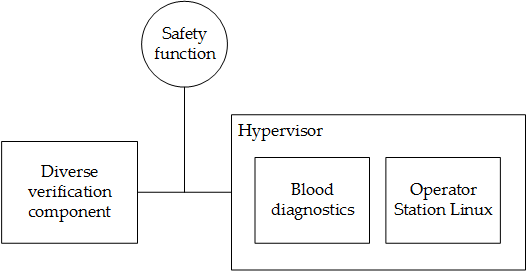
\includegraphics[scale=0.75]{Figures/blood_diagnostics_arch}
\decoRule
\caption{Example hypervisor partition setup}
\label{fig:blood_diagnostics_hv_arch}
\end{figure}

However, the system's need for fault tolerance means that some advanced fault tolerance techniques are necessary to mitigate the risks as much as possible. One way this could be achieved with a hypervisor architecture can be seen in figure \ref{fig:blood_diagnostics_hv_arch}. In this case both the safety-critical partition and the operator station partition are running on the hypervisor, with a secondary microcontroller performing the same calculations and verifying the output of the safety-critical hypervisor partition. Even though this means there are now multiple processors present, the hypervisor still provides consolidating effects. A pure \gls{HSS} architecture would still require a minimum of three partitions for the same setup.
% FIGURE Make an architecture figure 

% NOTE The proximity things seems like bullshit. Where did I even get that from?
If we assume that the separation is adequate and all basic safety requirements can be met, there are still factors left to consider. First of all, since this is a system that deals with real-time requirements, proximity to the machinery could be valuable. But in this case \gls{EMC} can cause significant issues. In the hypervisor setup a processor with a higher frequency would sit closer to the motors and other machinery which also themselves have \gls{EMI}. This could easily lead to a violation of the \gls{EMC} requirements of the regulatory body, introducing the need to add more electromagnetic shielding. 

This device can also benefit from the hypervisor's architectural improvements and easier configuration, perhaps even more so. Since it is more complex, it is also more likely that functionality can be usefully extracted into partitions, carrying the benefits explained in \ref{Chapter4}. But it is important to keep in mind that for a device with these characteristics, some of the typical hypervisor benefits are less relevant.

First of all, the hardware cost savings are not going to make a big impact on a device this complex and big. Secondly, \gls{SWaP} are also not as crucial as for the portable gas detector. The housing of this unit is already going to be at least as big as a typical wardrobe and an extra microcontroller is not going to change that. Same goes for weight. And since the device is connected to power all the time, making it as power efficient as possible is also not a primary goal.

\begin{comment}
% NOTE Did I say it is necessary in the introduction?! If not why am I arguing about his here. Bad section
One last thing that needs to be kept in mind is the typical hypervisor's current hardware restrictions. If a \gls{DSP} is necessary to control the device, the hypervisor could be at a disadvantage, since there is currently no \gls{DSP} that can host a hypervisor. But this may change [source] in the near future.  
\end{comment}

\subsubsection{Conclusion}
This example represents a high complexity, high criticality project that can already profit from the more traditional approaches of separation but where, in a reevaluation of device architecture, the hypervisor approach might come out on top. 

Some of the hypervisor benefits are not as important as in other classes of devices but it might still be an overall better choice, if the other factors like \gls{EMC} and safety of separation can be adequately satisfied. This example has of course been significantly simplified to construct a discussion about devices that are in this range of complexity and criticality and in a real-world example a lot more analysis will be necessary to determine whether the hypervisor is a good fit. As of 2018 this may still be a risky technical decision but with the push into hypervisors by the aviation and automotive industry, industries that manufacturer exactly this class of devices, this could evaporate within the next decade.

%----------------------------------------------------------------------------------------

\section{How to decide on a hypervisor implementation} \label{how-to-decide}
% NOTE Maybe talk about how this applies to first-party hypervisors?
This section explores the extended analysis that needs to be carried out by the manufacturer, once he is seriously considering using a third-party hypervisor. For the most part, it consists of a list of questions that need to be asked, with further explanation, if required. The categorization of the questions closely resembles the key wants established in \ref{Chapter3}.

Actually, it is conceivable that the result of this analysis reveals that no third-party hypervisors exists that can satisfy the manufacturers targets. The importance of each question is going to vary on a project by project basis and questions should be asked roughly in their order of importance. 

\subsection{Certifiability}
\paragraph{Which level of criticality does the hypervisor developer claim to be able to certify to?}
Since, this section is concerned with the concrete real-world examples, the abstract concept of criticality levels also has to be abandoned. It only makes sense to ask this question in relation to the actual regulations that the device will be certified to.

\paragraph{What deliverables and services does he offer to aid with certification?}
Usually the developer will offer documentation and test cases for the hypervisor that can be presented as evidence of safety to the regulatory bodies. But typically there is more work to do: the specifics depend on the standard but at the very least the risk of using the hypervisor needs to be evaluated and justified. Developers will also usually offer services to help with the certification of the hypervisor. Depending on the manufacturer's prowess with the regulations and the hypervisor such a service could be worthwhile.
\paragraph{Has the hypervisor successfully been used in a device that has to comply to the same regulations?}
Although, a "proven-in use" status is not enough to convince a regulatory body of a piece of software's safety it is at least evidence, that it can be done.
\paragraph{Do the claims of the developer and his documentation survive more intense scrutiny and project specific risk analysis?}
Because the hypervisor developers are clearly trying to sell a product, their claims should be met with scrutiny. This is a question that should probably be analyzed in the latter stages of the decision process.
\subsection{Cost}
The question of the hypervisor license cost has been mostly avoided in this thesis, since it can't be answered on a general level. Now is the time to come back to it.
\paragraph{What license model is applicable and what will the license cost?}
License models tend to vary based on unit cost and rate of production.
The cost of the license is probably exclusively subject to negotiation. 
\paragraph{Is there functionality or services that cost extra? Are they desirable?}
One possibility for an extra service has already been listed; enlisting the developer to help with certification. But some, more specialized functionality may also be gated behind additional cost. Furthermore, the developers almost always offer general services surrounding the hypervisor: helping with configuration and developing more features being among them. Especially, developers of open-source hypervisors tend to sustain themselves this way.
\paragraph{What costs are associated with the operating system that will run on the hypervisor?}
This question doesn't necessarily have to do with the hypervisor developer directly, although it can. The default paravirtualized \gls{OS} is supplied by the hypervisor developer and may incur additional costs. If the manufacturer decides to customize an operating system himself or use a fully virtualized free open-source \gls{OS} these license costs can be avoided. 
\subsection{Dependence}
The last question in the previous section already hints at it: using a third-party hypervisor can introduce significant dependence to said third-party, especially sine the third-party also offers the \gls{OS} running on top of the hypervisor.
\paragraph{Is the hypervisor source code available?}
\paragraph{Is it feasible for the manufacturer to modify the hypervisor on his own?}
This requires the source code to be available and legally modifiable. Such actions could include supporting additional hardware and changing or adding hypervisor functionality. If the manufacturer is planning to build expertise with the hypervisor implementation this can allow him to save costs by not enlisting the original developer to fulfill these services.

\paragraph{What paravirtualized operating systems are available and can the manufacturer feasibly add new ones?}

\paragraph{If the device has real-time requirements, can they be met with the hypervisor architecture?}
This is clearly a very difficult question to answer, before development has even begun but it still needs to be analyzed to avoid disaster.
\subsection{Additional functionality}
The core functionality the hypervisor offers has been explored in \ref{Chapter2}. This section is concerned with slightly more advanced features. Some hypervisor implementations are completely bare-bones and offer nothing beyond the features of a basic hypervisors and others offer many advanced features. This difference is likely to be reflected in the price of the respective implementations.
\paragraph{What additional functionality can the developer offer?}
Below is a list of some possible features that exist in current implementations.
% NOTE Do any items require additional explanation?
\begin{itemize}
    \item Different possible scheduling policies
    \item Health monitoring
    \item Device pass-through (Requires an \gls{IOMMU} to work effectively)
    \item Full virtualization
    \item Virtual input device support
    \item Security [It seems pretty half-assed to just dump security here]
    \item Automatic tests during operation
    \item Virtual high resolution timers
\end{itemize}

\subsection{Impact on the development process}
\subsubsection{Tooling}
\paragraph{What tools are available for hypervisor configuration?}
The two possible categories of tools are \gls{CLI} and \gls{IDE} tools. A \gls{CLI} tool may take input directly or from configuration files in a specific format. An \gls{IDE} could instead offer a graphical representation with possible values, hints and even drag and drop configuration of some features. If done well this can greatly reduce the barrier of entry for new users, if done badly this can cloud the users understanding of the actual configuration and introduce errors.

Some regulations also require that all tools used to created safety-critical devices need to be verified and the same applies for the tools used to configure and build the hypervisor. It can be expected that an \gls{IDE} is more expensive to verify than a \gls{CLI} tool and while this may not impact the manufacturer directly, it may increase the cost of the hypervisor license.
\paragraph{What compilers and debuggers are supported and do they align with the project requirements?}
Compilers and potentially even debuggers need to be verified as well. This means that safety-critical device manufacturer typically use less common compilers that are already verified. If the hypervisor, for whatever reason, doesn't support that specific compiler it could incur additional cost or even render it infeasible.
\subsubsection{Debugging and tracing}
Since the hypervisor acts as a layer of abstraction between the hardware and software it has the potential to be a great aid in debugging the system. But simultaneously it could also act as a great hindrance, obfuscating issues in the business code and not providing access to partition data that would have been available without the hypervisor.
\paragraph{Does the hypervisor provide standard debugging functionality?}
There are multiple ways to achieve this and they will not be explored in detail here but the two most prominent examples are: a debugging server running on the device and a hypervisor aware \gls{JTAG} environment. Ideally, it is possible to debug both the hypervisor and the guest operating systems independently. [source to hypervisors that do this and lauterbach ad]
\paragraph{Does the hypervisor provide special debugging or tracing functionality?}
As established in section \ref{distributed-or-centralized}, the hypervisor has a unique centralized view of the system. It can therefore expose its internal events to a developer and provide high level insight into what exactly is happening inside the hypervisor.

%----------------------------------------------------------------------------------------

\section{Noteworthy implementations} \label{noteworthy-implementations}
As a contrast to the "basic safety-hypervisor" established early in the thesis, now will be given some notable 2018 implementations. Keep in mind that no claim is being made about their respective quality, it is just being pointed out what interesting and unique features or characteristics they have.
\subsection{seL4 and CAmkES} \label{seL4}
seL4 is a formally verified microkernel with a focus on security, so far it has been mostly confined to academia but some advances into real products have been made since [source]. \textquote{CAmkES (component architecture for microkernel-based embedded systems) is a software development and runtime framework for quickly and reliably building microkernel-based multiserver (operating) systems.}[source]. A system that is built with these two can also host virtual machines on some platforms. This implementation provides much more flexibility than a basic hypervisor, as it can be used to design general modular software systems. The formal verification of seL4 and CAmkES, as well as the additional verification output that can be generated automatically, can go a long way in certifying a safety-critical device.
% Link CAmkES source: https://docs.sel4.systems/CAmkES/
\subsection{SYSGO's PikeOS}
PikeOS is unique because it is a real-time operating system first and foremost with hypervisor functionality added on top. Similar to seL4 with CAmkES it can provide much more flexibility in designing the system than a hypervisor that offers only virtualized guest environments. Partitions can host \gls{RTOS} task trees or a virtualized operating system respectively. This also eliminates the need to virtualize an \gls{RTOS} in the first place.

Additionally, PikeOS offers a form of hierarchical scheduling which can make the scheduling of mixed criticality systems more efficient and potentially easier [source].
\subsection{OpenSynergy's COQOS MICRO SDK}
* (LynxSecure)
* Mentor (as a really small example, maybe find additional)
* PROVENVISOR (formally verified, security focus)
* GreenHills, WindRiver and maybe QNX as "expensive high-profile" hypervisors
* [...] 
% Chapter 1

\chapter{Conclusion and Future considerations} % Main chapter title

\label{Chapter6} % For referencing the chapter elsewhere, use \ref{Chapter1} 

%----------------------------------------------------------------------------------------

% Define some commands to keep the formatting separated from the content 
%\newcommand{\keyword}[1]{\textbf{#1}}
%\newcommand{\tabhead}[1]{\textbf{#1}}
%\newcommand{\code}[1]{\texttt{#1}}
%\newcommand{\file}[1]{\texttt{\bfseries#1}}
%\newcommand{\option}[1]{\texttt{\itshape#1}}

%----------------------------------------------------------------------------------------

\section{Further research}
\paragraph{Analyzing the cost of hypervisor licenses}
While the true cost of a typical hypervisor license will likely continue to elude further because of the developer's secrecy, an educated estimation could likely be produced. If you look at the market of hypervisor implementation, there appears to be the typical pattern of luxury solutions and basic solutions. A cost analysis of these categories based on known factors, like lines of code and list of features, while likely to be somewhat inaccurate would help immensely to quantify the difference between the \acrshort{hss} and the hypervisor architecture.
\paragraph{Quantifying the theoretical analysis proposed in this thesis}
Most of the points made in chapter \ref{Chapter4} are based on logical argumentation and only highlight possibilities. Quantifying some or all of these claims would grant deeper insight into the hypervisor benefits and drawbacks.
%----------------------------------------------------------------------------------------

\section{Technological progress} \label{tech-progress}
\subsection{New hardware platforms} \label{cortex-r52-hypervisor}
Probably the most notable development already on the horizon is the newest member of the ARMv8-R architecture. The ARMv8-R architecture is specifically designed for safety-critical environments with real-time requirements \cite{armr}. 
The Cortex-R52 specification has been released in 2017 \cite{armcortexr52}, and now the first silicon implementations are going into preproduction \cite{nxp}. It offers eight logical cores operating in dual-core lock step, multiple safety features, and typical \acrshort{dsp} functionality. Unusually for a microcontroller of this scope, it also contains an \acrshort{mpu} and hardware virtualization extensions. Furthermore, there is already an unreleased hypervisor that takes advantage of this new platform \cite{opensynergy}. This means that in the future the concerns with using application processors in real-time safety-critical devices will no longer apply because low-powered microcontrollers will be able to support virtualization.

\subsection{Sophistication of technology}
Relatively speaking, embedded virtualization and safety-critical hypervisors are a very new technology. Once these technologies are used in more products and mature with their challenges a lot of the problems, established in this thesis will hopefully be proven obsolete, while the benefits will be even more pronounced. 

The same is probably true for the alternative architectures that were introduced in chapter \ref{Chapter1} but not further analyzed.
\subsection{Advances in formal verification}
As seL4 and some of the associated research show, formal verification is becoming increasingly viable for actual products \cite{sel4faq}. Especially, with the advent of tools that can automatically create the required proofs, formal verification is becoming feasible for developers with no research background in the field of formal verification. This development may not only have implications for safety hypervisors but for safety-critical engineering as a whole.

%----------------------------------------------------------------------------------------

\section{Conclusion}
Certifying components to the lowest possible criticality level instead of the highest criticality present in the device is very desirable for an efficient development process. To be able to do this it is necessary to provide evidence of an appropriate separation of components. A device architecture that solves this problem of mixed-criticality has been introduced as a separation architecture.

Historically speaking the only architecture that was capable of this separation, was the hardware separated subsystems architecture. In this architecture, additional processors, along with other necessary resources, are added to the system to separate the components from each other. If a safety-critical device manufacturer can solve the mixed criticality problem cheaper and make it feasible in smaller devices, it could be a significant edge over competitors.

The primary contender for this better separation architecture is the embedded safety hypervisor. It typically consists of a microkernel which can host both native C runtimes and, to give the hypervisor its name, virtualized operating systems. Because it has already been gaining traction in the automotive industry and some outliers in other sectors, this architecture is also what this thesis set out to analyze. Chapter \ref{Chapter2} introduced a basic safety hypervisor that displays all the functionality of common hypervisor implementations. The features that can probably achieve the greatest value for the manufacturer were health monitoring and multicore support. Multicore support is a valuable tool for achieving maximum hardware consolidation. Health monitoring can be used to detect abnormal system events and react appropriately. 

% TODO Make what I write here clear in the respective introduction.
As a way to abstract the business goals of safety-critical device manufacturers, their \keyword{key wants} were introduced. These later served as categorization for the comparative analysis of the two architectures. And although the importance of each category was not explored fully, they should allow an eventual safety-critical device engineer to understand which are most important for his device. Consequently, it can be used to judge the importance of certain architecture benefits and drawbacks.

% NOTE In the current structure they did not emerge from it, crucial differences come first.
Through the theoretical analysis in chapter \ref{Chapter4}, some crucial differences between the architectures emerged:
\begin{itemize}
    \item The hypervisor's separation cannot surpass that of the \acrshort{hss} architecture.
    \item Hypervisor is more modifiable and can provide smaller utility features.
    \item Hypervisor is a reusable, general solution, so costs are shared between parties over a period of time.
    \item Hypervisor's centralized view give it unique opportunities for system management and fault tolerance.
    \item Hypervisor partitions are cheaper to add and can, therefore, help achieve a more modular device architecture.
\end{itemize}

% IMPORTANT Update this if I decide to add another reference project.
The reference projects of section \ref{ref-projects} introduced two broad categories of safety-critical devices that could benefit from the hypervisor architecture. In the first device category, separation is becoming increasingly important because of growing user demands but the traditional \acrshort{hss} architecture cannot fulfill the requirements of the manufacturer. These devices are often hand-held and battery powered and are consequently very sensitive to negative changes in size, weight, and power. All of which are negatively impacted by the \acrshort{hss} architecture.
Devices of this scope are also more likely to be produced in larger quantities, so the added hardware cost of a second processor would be quite undesirable. This project was also used as the basis of an extensive example hypervisor configuration.

The second device category was one of much higher complexity, where a separation architecture would even be used if the hypervisor was not available. Devices in this category will often have more stringent regulations to follow, so the manufacturer will have a harder time deploying a hypervisor compared to the \acrshort{hss} architecture. But if these challenges can be overcome, the hypervisor architecture can provide hardware consolidation and a more future-proof device.

Finally, the questions proposed in section \ref{how-to-decide} give a concrete list of criteria to evaluate before moving on to use the hypervisor architecture in a real-world project. To paraphrase the broad categories of questions:
\begin{itemize}
    \item Can the device, including the hypervisor, be feasibly certified for the required regulations?
    \item How much does the hypervisor impact unit cost overall?
    \item How dependent would the device manufacturer be on the hypervisor developer?
    \item Can the hypervisor offer the necessary performance?
    \item Can the hypervisor offer additional functionality that would be particularly valuable?
    \item How does the hypervisor impact the development process?
\end{itemize}
Along with the noteworthy hypervisor implementations of section \ref{noteworthy-implementations} and the reference projects this should give the safety-critical device engineer, plenty of information to base his analysis on. 

The hypervisor architecture for safety-critical devices is still young and connected to a lot of uncertainty, but given time, these issues are surmountable. It is unlikely to be a complete replacement for hardware-based separation architectures like the \acrshort{hss} architecture, but there is bound to be a broad device category where it can outperform the traditional architectures.


\begin{comment} 
* Mixed criticality has been present for a long time in very complex projects but with increased processing power and user demands it makes more and more sense in smaller devices.
* For this reason and because of efforts in some industries to save SWaP alternate solutions to the mixed criticality problem have been seeing some adoption.
* One of these is the hypervisor that this thesis set out to compare more in-depth.
* From that comparison the crucial differences and their effects emerged
* [Refer to conclusion from that section]
* Based on this some reference project have been proposed that can be categorized into these [] categories.
* Ultimately it can be said the hypervisor has a couple of very promising places of application.
* So it can be said the best scenarios for the hypervisor architecture are the ones where this happens: []
* The advent of microkernel based safety hypervisors along with the maturation in virtualization technology, especially in the embedded space provides an avenue to deal with the problems that arise from mixed criticality.
\end{comment}
 

%----------------------------------------------------------------------------------------
%	THESIS CONTENT - APPENDICES
%----------------------------------------------------------------------------------------
\begin{comment}

\appendix % Cue to tell LaTeX that the following "chapters" are Appendices

% Include the appendices of the thesis as separate files from the Appendices folder
% Uncomment the lines as you write the Appendices

%% Appendix A

\chapter{Frequently Asked Questions} % Main appendix title

\label{AppendixA} % For referencing this appendix elsewhere, use \ref{AppendixA}

\section{How do I change the colors of links?}

The color of links can be changed to your liking using:

{\small\verb!\hypersetup{urlcolor=red}!}, or

{\small\verb!\hypersetup{citecolor=green}!}, or

{\small\verb!\hypersetup{allcolor=blue}!}.

\noindent If you want to completely hide the links, you can use:

{\small\verb!\hypersetup{allcolors=.}!}, or even better: 

{\small\verb!\hypersetup{hidelinks}!}.

\noindent If you want to have obvious links in the PDF but not the printed text, use:

{\small\verb!\hypersetup{colorlinks=false}!}.

%\include{Appendices/AppendixB}
%\include{Appendices/AppendixC}
\end{comment}

%----------------------------------------------------------------------------------------
%	BIBLIOGRAPHY
%----------------------------------------------------------------------------------------

\printbibliography[heading=bibintoc]

%----------------------------------------------------------------------------------------

\end{document}  
